\RequirePackage{silence}
\WarningFilter{titlesec}{Non standard sectioning command}
\WarningFilter{scrreprt}{Usage of package}
\WarningFilter{scrreprt}{Activating an ugly workaround}

% **************************************************
% Document Class Definition
% **************************************************
\documentclass[%
	paper=A4,					% paper size --> A4 is default in Germany
	twoside=true,				% onesite or twoside printing
	openright,					% doublepage cleaning ends up right side
	parskip=full,				% spacing value / method for paragraphs
	chapterprefix=true,			% prefix for chapter marks
	11pt,						% font size
	headings=normal,			% size of headings
	bibliography=totoc,			% include bib in toc
	listof=totoc,				% include listof entries in toc
	titlepage=on,				% own page for each title page
	captions=tableabove,		% display table captions above the float env
	draft=false,				% value for draft version
]{scrreprt}%

% **************************************************
% Debug LaTeX Information
% **************************************************
%\listfiles

% **************************************************
% Information and Commands for Reuse
% **************************************************
\newcommand{\thesisTitle}{Boosting methods for refining diffusion models}
\newcommand{\thesisName}{Ahmed Mehdi Inane}
\newcommand{\thesisSubject}{Master's thesis}
\newcommand{\thesisDate}{August 28, 2024}
\newcommand{\thesisVersion}{Reviewer's version}

\newcommand{\thesisFirstReviewer}{Etienne Decencière}
\newcommand{\thesisFirstReviewerUniversity}{\protect{Ecole des Mines de Paris,PSL}}
\newcommand{\thesisFirstReviewerDepartment}{Centre de morphologie mathématique}

\newcommand{\thesisSecondReviewer}{Gabriel Peyr\'e}
\newcommand{\thesisSecondReviewerUniversity}{\protect{Ecole Normale Supérieure}}
\newcommand{\thesisSecondReviewerDepartment}{Département de Mathématiques et Applications}

\newcommand{\thesisFirstSupervisor}{Alexandre V\'erine}
\newcommand{\thesisSecondSupervisor}{Yann Chevaleyre}

\newcommand{\thesisUniversity}{\protect{Universit\'e Paris-Dauphine}}
\newcommand{\thesisUniversityDepartment}{LAMSADE}
\newcommand{\thesisUniversityGroup}{Machine Intelligence and Learning Systems (MILES)}
\newcommand{\thesisUniversityCity}{Paris}
\newcommand{\thesisUniversityStreetAddress}{Place du Maréchal de Lattre de Tassigny}
\newcommand{\thesisUniversityPostalCode}{75016}

% **************************************************
% Load and Configure Packages
% **************************************************
\usepackage[utf8]{inputenc}		% defines file's character encoding
\usepackage[english]{babel} % babel system, adjust the language of the content
\usepackage[					% clean thesis style
	figuresep=colon,%
	sansserif=false,%
	hangfigurecaption=false,%
	hangsection=true,%
	hangsubsection=true,%
	colorize=full,%
	colortheme=bluemagenta,%
% LLT: Use biber if using UTF8 encoding
 	bibsys=bibtex,%
%	bibsys=biber,%
	bibfile=bib-refs,%
	bibstyle=alphabetic,%
]{cleanthesis}
\usepackage{amsthm}
\usepackage{amsmath}
\usepackage{amssymb}
\usepackage{array} 
\usepackage{algorithm}
\usepackage{algpseudocode}
\usepackage{multicol}
\usepackage{booktabs}
\usepackage{subcaption}
\hypersetup{					% setup the hyperref-package options
	pdftitle={\thesisTitle},	% 	- title (PDF meta)
	pdfsubject={\thesisSubject},% 	- subject (PDF meta)
	pdfauthor={\thesisName},	% 	- author (PDF meta)
	plainpages=false,			% 	-
	colorlinks=false,			% 	- colorize links?
	pdfborder={0 0 0},			% 	-
	breaklinks=true,			% 	- allow line break inside links
	bookmarksnumbered=true,		%
	bookmarksopen=true			%
}

\usepackage{notation}

% **************************************************
% Document CONTENT
% **************************************************
\begin{document}

\newtheoremstyle{myassumption} % Name of the style
  {3pt} % Space above
  {3pt} % Space below
  {\itshape} % Body font
  {} % Indent amount
  {\bfseries} % Theorem head font
  {.} % Punctuation after theorem head
  {.5em} % Space after theorem head
  {} % Theorem head spec (can be left empty, meaning ‘normal’)

% Applying the style to the 'assumption' environment
\theoremstyle{myassumption}
\newtheorem{assumption}{Assumption}
\newtheorem{definition}{Definition}
\newtheorem{theorem}{Theorem}
\newtheorem{lemma}{Lemma}
\newtheorem{proposition}{Proposition}

% --------------------------
% rename document parts
% --------------------------
%\renewcaptionname{ngerman}{\figurename}{Abb.}
%\renewcaptionname{ngerman}{\tablename}{Tab.}
\renewcaptionname{english}{\figurename}{Fig.}
\renewcaptionname{english}{\tablename}{Tab.}

% --------------------------
% Front matter
% --------------------------
\pagenumbering{roman}			% roman page numbing (invisible for empty page style)
\pagestyle{empty}				% no header or footers
% !TEX root = ../thesis-example.tex
%
% ------------------------------------  --> cover title page
\begin{titlepage}
	\pdfbookmark[0]{Cover}{Cover}
	\flushright
	\hfill
	\vfill
	{\LARGE\thesisTitle \par}
	\rule[5pt]{\textwidth}{.4pt} \par
	{\Large\thesisName}
	\vfill
	\textit{\large\thesisDate} \\
	Version: \thesisVersion
\end{titlepage}


% ------------------------------------  --> main title page
\begin{titlepage}
	\pdfbookmark[0]{Titlepage}{Titlepage}
	\tgherosfont
	\centering

	{\Large \thesisUniversity} \\[4mm]
	
\includegraphics[width=6cm]{gfx/logo_dauphine.png} \\[2mm]
	\textsf{\thesisUniversityDepartment} \\
	\textsf{\thesisUniversityInstitute} \\
	\textsf{\thesisUniversityGroup} \\

	\vfill
	{\large \thesisSubject} \\[5mm]
	{\LARGE \color{ctcolortitle}\textbf{\thesisTitle} \\[10mm]}
	{\Large \thesisName} \\

	\vfill
	\begin{minipage}[t]{.27\textwidth}
		\raggedleft
		\textit{1. Supervisor}
	\end{minipage}
	\hspace*{15pt}
	\begin{minipage}[t]{.65\textwidth}
		{\Large \thesisFirstSupervisor} \\
		{\small \thesisUniversityGroup} \\[-1mm]
		{\small \thesisUniversity}
	\end{minipage} \\[5mm]
	\begin{minipage}[t]{.27\textwidth}
		\raggedleft
		\textit{2. Supervisor}
	\end{minipage}
	\hspace*{15pt}
	\begin{minipage}[t]{.65\textwidth}
		{\Large \thesisSecondSupervisor} \\
		{\small \thesisUniversityGroup} \\[-1mm]
		{\small \thesisUniversity}
	\end{minipage} \\[10mm]
	\thesisDate \\

\end{titlepage}


% ------------------------------------  --> lower title back for single page layout
\hfill
\vfill
{
	\small
	\textbf{\thesisName} \\
	\textit{\thesisTitle} \\
	\thesisSubject, \thesisDate \\
	Reviewers: \thesisFirstReviewer\ and \thesisSecondReviewer \\
	Supervisors: \thesisFirstSupervisor\ and \thesisSecondSupervisor \\[1.5em]
	\textbf{\thesisUniversity} \\
	\textit{\thesisUniversityGroup} \\
	\thesisUniversityInstitute \\
	\thesisUniversityDepartment \\
	\thesisUniversityStreetAddress \\
	\thesisUniversityPostalCode\ and \thesisUniversityCity
}
		% INCLUDE: all titlepages
\cleardoublepage

\pagestyle{plain}				% display just page numbers
% !TEX root = ../thesis-example.tex
%
\pdfbookmark[0]{Abstract}{Abstract}
\chapter*{Abstract}\label{sec:abstract}
\vspace*{-10mm}
This thesis work presents two methods in refining the generation of generative models, particularly diffusion models.
Popular generative models typically contain billions of parameters. They incur a hefty training cost, in both energy and time, and the architecture choice often restrict the estimation to have a suboptimal estimation of the target distribution.
\\
As a result, we are interested in ways to boost generative models with smaller models, in order to mitigate generation errors, due to either estimation or sampling. Focusing our work on diffusion models, we thus propose two methods : improved discriminator guidance, which consists in using a discriminator to correct the estimation error, and f-Policy gradient, which circumvents the errors induced by solving the backward SDE of a diffusion process by using reinforcement learning and dense signals provided by measuring the f-divergence between the two distributions.
\\ 
We provide theoretical guarantees proving the validity of our methods and demonstrate their effectiveness on standard benchmark datasets. Our experiments show that boosting improves the generation process without incurring a substantial cost that would otherwise be obtained by fine-tuning the model.
\vspace*{20mm}

		% INCLUDE: the abstracts (english and german)
\cleardoublepage
%
% !TEX root = ../thesis-example.tex
%
\pdfbookmark[0]{Acknowledgement}{Acknowledgement}
\chapter*{Acknowledgement}\label{sec:acknowledgement}
\vspace*{-10mm}
Many thanks to Alex for teaching me so many things, and for allowing such a great collaboration to happen. I thank him for his patience, enthusiasm and for setting up a great learning environment. You have been a great mentor !
I thank Yann for trusting me with this research project, and for providing meaningful advice and insightful mathematical observations. 
\\
During this internship, I worked at the MILES team, and I would like to thank all my colleagues that made this research experience incredible. A special mention to Matteo and Augustin for quality coffee breaks, Lucas and Erwan for their sound advice, and to all the team for their support and kindness.
\\
Finally, I would like to thank my family and friends for their support and encouragement during this internship. Thank you Carla for being there for me.
\\
This work has inspired me to continue research within machine learning, and I hope it will be the first of many more to come.

 % INCLUDE: acknowledgement
\cleardoublepage
%
\setcounter{tocdepth}{2}		% define depth of toc
\tableofcontents				% display table of contents
\cleardoublepage

% --------------------------
% Body matter
% --------------------------
\pagenumbering{arabic}			% arabic page numbering
\setcounter{page}{1}			% set page counter
\pagestyle{maincontentstyle} 	% fancy header and footer

% !TEX root = ../thesis-example.tex
%
\chapter{Introduction}\label{sec:intro}
During the past decade, the use of artificial intelligence (AI) and machine learning (ML) methods has spread across various sectors, driving innovation and efficiency at unprecedented scales.
The development of hardware components such as Graphical Processing Units (GPUs) and Tensor Processing Units (TPUs), combined with the availability of large amounts of data has shown the potential of Machine Learning models to uncover latent patterns in data, and has 
driven advancements in fields such as image and natural language processing, autonomous driving, healthcare, and finance. A particular class of ML models, termed as generative modeling, has shown promise in the recent years by its ability to generate realistic samples by training on a dataset.
\\
Generative modeling is a subfield of machine learning that focuses on learning the underlying distribution of a dataset to generate new samples. It has proven to be effective for numerous types of data, including language \citep{openai2024gpt4technicalreport}, image generation \citep{rombach2022highresolutionimagesynthesislatent}, and drug discovery \citep{jumper2021highly}.
Recent generative models are based on neural networks, and prominent models include Generative Adversarial Networks (GANs) \citep{goodfellow2014generativeadversarialnetworks}, Variational Auto-Encoder (VAEs) \citep{Kingma_2019}, and Diffusion models \citep{song2021scorebasedgenerativemodelingstochastic}.
\\
The success of generative models hides their training procedure that is usually long, computationally expensive, and requires a large amount of data. The training of generative models is challenging due to the high-dimensional nature of the data and the need to learn complex distributions. For instance, figure \ref{fig:expo_parameters} displays an exponential increase on the number of parameters of architectures involved in generative models.
This raises numerous questions on the \textit{frugality} of the training procedure. Several research directions have been proposed to address this issue, including the use of transfer learning \citep{zhuang2020comprehensivesurveytransferlearning}, neural architecture search \citep{verbockhaven2024growingtinynetworksspotting} and pruning methods \citep{sun2024simpleeffectivepruningapproach}.
\begin{figure}[t]
    \centering
    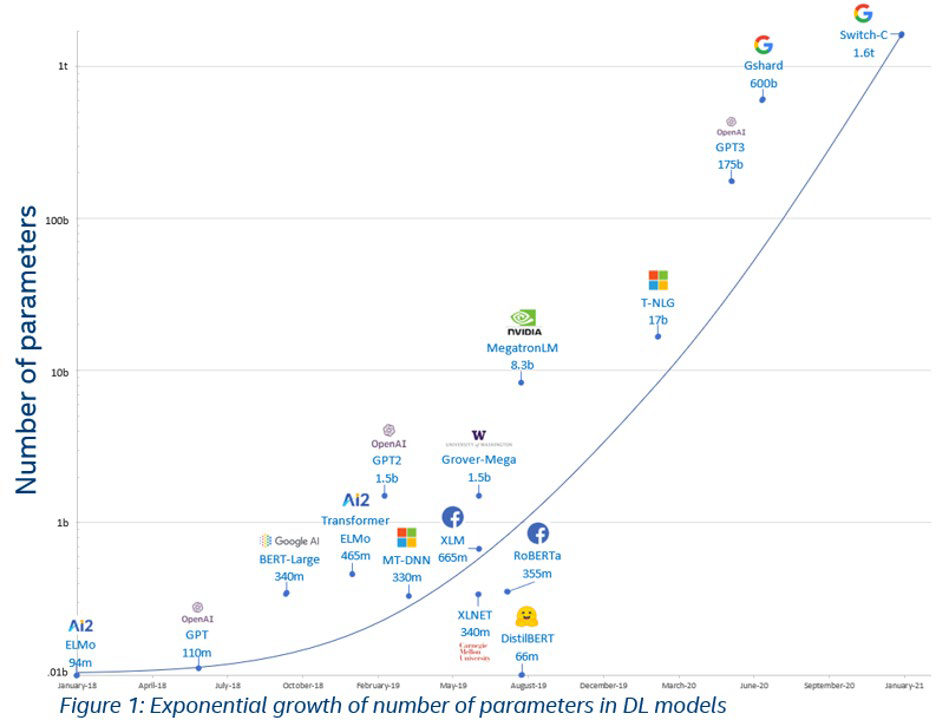
\includegraphics[width=\textwidth]{gfx/expo_parameters.png}
    \caption{Number of parameters of architectures used in large language models. Source: \url{https://www.webagesolutions.com/blog/generative-ai-engineering}}
    \label{fig:expo_parameters}
\end{figure}
\\

In this work, we focus on a subset of generative models, that is diffusion models. Diffusion models consists in 
gradually adding noise to the data and then learning to reverse this process to reconstruct the original data. This type of model has gained attention for its potential to generate high-quality and diverse samples, while providing a theoretically sound framework based on Markov chains \citep{ho2020denoisingdiffusionprobabilisticmodels} and stochastic differential equations \citep{song2021scorebasedgenerativemodelingstochastic}. 
We are particularly interested in developing methods to refine a pre-trained diffusion model without re-training it. That is, improve its generation abilities without using the important computational power required to train the whole model.
More specifically, we aim to investigate the potential of using boosting methods, i.e using auxiliary smaller models, to improve the generation capabilities of a pre-trained diffusion model. A smaller model will thus act as correcting the errors made by the pre-trained model. 
\\
The main sources of error that a diffusion model can make stem from \textit{approximation} erros and \textit{sampling} errors. Approximation errors denote the accuracy of estimation of the score compnent during the training phase, and sampling errors refer to the errors made during the sampling phase. 
We thus raise the following question : 
\begin{center}
    \textbf{Can we devise boosting methods to correct the errors made by a pre-trained diffusion model ?}
\end{center}
We answer to this question by presenting two methods : discriminator guidance and f-Restart sampling. The former method attemps to correct the approximation error by using a smaller discriminator network to correct the score. f-Restart sampling attempts to correct the sampling error by using a reinforcement learning procedure during the sampling process, deciding between performing a denoising step or injecting noise as a correction term.
The structure of our thesis is as follows : \begin{itemize}
    \item \textbf{Chapter \ref{sec:diffusion} :} In this section, we give an overview of generative models, then present the derivation of diffusion models. Then, we list a few refinement methods proposed for generative models that are based on density ratio estimation technique, motivating the use of a discriminator.
    \item \textbf{Chapter \ref{sec:dg} :} In this section, we present discriminator guidance as a method for correcting the approximation error involved in training a score network. We improve upon previous results by deriving an optimal objective function, and we expose the experimental results on standard image generation benchmarks.
    \item \textbf{Chapter \ref{sec:rl} :} In this section, we present restart sampling as a boosting-free method for refining the sampling error of a diffusion model. We then propose $f-$Restart sampling, a method that improves upon the previous one by incorporating a reinforcement learning algorithm to dynamically denoise samples.
\end{itemize}
 % INCLUDE: introduction
% !TEX root = ../thesis-example.tex
%
\chapter{Background}\label{sec:diffusion}

This chapter introduces the necessary background that is relevant to our work. In the following, we provide an overview of generative modeling methods in machine learning. Then, we present diffusion models as the generative method we would like to improve. Finally, we present a few density ratio estimation techniques as this will be the backbone of our refinement techniques. 

\section{Generative modeling}\label{sec:related:sec1}


Generative modeling denotes a branch of unsupervised learning that aims to construct a \textbf{model} of the data $x \in \mathcal{X}$. By considering that a dataset can be described by a probability distribution $p(x)$ - that we call a \textit{target} distribution - the challenge is to estimate such a distribution by finding the best set of parameters able to approximate it, among a set of potential \textit{generators} $G$. A notable ability of generative models is generating new data instances that resemble the observed data, by sampling from the \textit{estimated} distribution $\hat{p}(x)$ .
Through the rapid development of deep learning and the abundance of training data over the past decade, generating data has attained impressive performances across various data types, often in high dimensions, such as language \citep{openai2024gpt4technicalreport}, visual data such as images \citep{rombach2022highresolutionimagesynthesislatent} and videos \citep{videoworldsimulators2024}, and speech \citep{wavenet}. This progress went on to include different types of input, termed as multimodal generative models \citep{Suzuki_2022}.

\subsection{Theoretical formulation}
\begin{assumption}\label{ass:1}
    We assume that the domain of interest $\mathcal{D} \subset \mathcal{X}$ is governed by a probability distribution  $P_{\mathcal{D}}$ of density $p(x)$.
\end{assumption}
Given a training dataset \textbf{x} of $n$ points sampled i.i.d from $P_{\mathcal{D}}$, we would like to approximate the target density $p(x)$ with a parametric family of models. Our focus is on deep learning based approaches involving neural networks. Thus, given a foxed architecture, we denote by $\Theta$ the set of all weights represented by this architecture.
The traditional approach in density estimation with a parametric family of models is maximum likelihood estimation (MLE) or maximum a posteriori (MAP). The likelihood function $L(\theta \mid X)$ of a parameter $\theta \in \Theta$ given the data $X$ is defined as the joint probability of the observed data:
\begin{equation}
L(\theta \mid X) = \prod_{i=1}^n p(x_i \mid \theta).
\end{equation}

The maximum likelihood estimation problem involves finding the parameter $\theta$ that maximizes the likelihood function. Formally, we define the MLE of $\theta$ as:
\begin{equation}
\hat{\theta}_{\text{MLE}} = \arg\max_{\theta} L(\theta \mid X).
\end{equation}

In practice, it is often more convenient to work with the log-likelihood function, since the logarithm is a monotonic function. The log-likelihood of $\theta$ is given by:
\begin{equation}
\ell(\theta \mid X) = \log L(\theta \mid X) = \sum_{i=1}^n \log p(x_i \mid \theta).
\end{equation}

Thus, the MLE problem can also be formulated as maximizing the log-likelihood:
\begin{equation}
\hat{\theta}_{\text{MLE}} = \arg\max_{\theta} \ell(\theta \mid X).
\end{equation}
This problem can be generalized as a \textbf{density estimation} problem, using the concept of statistical divergences.
\begin{definition}\label{def:divergence}
    Given two probability distributions $P,Q$ over $\mathcal{X}$, a statistical divergence $D(.\|.)$ is a function :
    \begin{equation}
D(P \| Q) : \mathcal{P} \times \mathcal{Q} \rightarrow [0, \infty),
\end{equation}
where $\mathcal{P}$ and $\mathcal{Q}$ are the spaces of probability distributions on $\mathcal{X}$.

The function $D(P \| Q)$ satisfies the following properties:
\begin{itemize}
  \item Non-negativity: $D(P \| Q) \geq 0$ for all $P, Q \in \mathcal{P} \times \mathcal{Q}$.
  \item Identity of indiscernibles: $D(P \| Q) = 0$ if and only if $P = Q$ almost everywhere.
\end{itemize}
\end{definition}
The absence of the symmetry assumption excludes statistical divergences from being metrics. However, they are still effective in comparing probability distributions. Table \ref{tab:divergences} provides examples of statistical divergences of interest in our work.
\begin{table}[ht]
\centering
\caption{Generic Mathematical Expressions for Statistical Divergences}
\[
\begin{array}{|>{\bfseries}m{4cm}|m{10cm}|}\label{tab:divergences}
\hline
\textbf{Category} & \textbf{Generic Mathematical Expression} \\
\hline
\textbf{F-Divergences} & $D_f(P \| Q) = \int q(x) f\left(\frac{p(x)}{q(x)}\right) \, dx$ \\
\hline
\textbf{Renyi Divergences} & $D_{\alpha}(P \| Q) = \frac{1}{\alpha - 1} \log \int p(x)^\alpha q(x)^{1-\alpha} \, dx$ \\
\hline
\textbf{Bregman Divergences} & $D_\phi(\mathbf{p}, \mathbf{q}) = \phi(\mathbf{p}) - \phi(\mathbf{q}) - \langle \nabla \phi(\mathbf{q}), \mathbf{p} - \mathbf{q} \rangle$ \\
\hline
\end{array}
\]
\end{table}
Given a divergence $D$, a target density $p(x)$ and a family of parametric models $\Theta$, one can formulate the optimal density as the solution of :
\begin{equation}\label{eq:density_est}
    \hat{\theta} = \arg\min_{\theta \in \Theta} D(\hat{p}(x; \theta) \| p(x))
\end{equation}
Once the density is estimated, one can sample from a generator $G_{\hat{\theta}}$ function, according to the type of generative model used.
\subsection{Sampling from an estimated distribution}
In this subsection, we give three examples of the training and sampling schemes of popular generative models in deep learning.
\begin{itemize}
    \item \textbf{Generative adversarial networks (GANs)} \citep{goodfellow2014generativeadversarialnetworks} consist in simultaneaous training of two different networks having opposing objectives. The first network, called a discriminator $D_{\phi}$ discriminates between samples from the \textit{target} distribution and samples from another distribution. The second network, called a generator $G_{\theta}$, attempts to sample from the target distribution to fool the discriminator. Essentially, this consists in solving the following min-max problem \citep{nowozin2016fgantraininggenerativeneural}, given a convex, lower-semi continuous function $f$:
    \begin{equation}\label{eq:f_gan}
        \min_{\theta} \max_{\phi} V(D_{\phi}, G_{\theta}) = \mathbb{E}_{x \sim p(x)}[D_{\phi}(x)] - \mathbb{E}_{z \sim p_{\theta}(z)}[f^*(D_{\phi}(G_{\theta}(z)))]
    \end{equation}
    where $f^*$ denotes the Fenchel conjugate of $f$. This objective function corresponds to a variational lower bound on the $f$-divergence between the target distribution and the generator distribution \citep{Nguyen_2010}. Once this objective is optimized, the generator $G_{\theta}$ is then used to sample from the estimated distribution. While GANs are celebrated for their sample quality, they often suffer from mode collapse which leads to a lack of diversity \citep{10.1145/3283254.3283282},and an unstable training due to the double optimization induced by the training objective.
    \item \textbf{Variational autoencoders (VAEs)} \citep{kingma2022autoencodingvariationalbayes} are probabilistic generative models that frame the problem of data generation as a Bayesian inference task. The key idea is to encode inputs into a latent (hidden) space via a neural network, and then decode from this latent space back to the data space. The encoder learns a distribution $q_{\phi}(z|x)$ over the latent space conditioned on the input data $x$, aiming to approximate the true but intractable posterior $p(z|x)$. The decoder, parameterized by $\theta$, attempts to reconstruct the input $x$ from the latent variable $z$, sampled from $q_{\phi}(z|x)$. The loss function of a VAE can be described as:
    \begin{align}
        \mathcal{L}(\theta, \phi; x) = -\mathbb{E}_{q_{\phi}(z|x)}[\log p_{\theta}(x|z)] + D_{\text{KL}}(q_{\phi}(z|x) \| p(z)),
    \end{align}
    where the first term is the expected log likelihood of the decoder (which measures reconstruction accuracy), and the second term is the Kullback-Leibler divergence between the encoded distribution and a prior distribution (typically a standard normal), acting as a regularizer. The VAE thus balances between accurate reconstruction and a meaningful, well-structured latent space. Sampling from a VAE involves passing randomly drawn samples from the prior $p(z)$ through the decoder to generate new data points that resemble the training data. As opposed to GANs, VAEs have a mass covering advantage but lack the quality provided by GAN generated samples. A recent line of work attempts to combine both strengths of these models to provide both quality and diversity to the generation process \citep{gimenez2022unifiedfdivergenceframeworkgeneralizing}.
    \item  \textbf{Diffusion Models} are another class of generative models that have recently gained significant attention due to their ability to generate high-quality samples. Similar to VAEs, diffusion models operate over a latent space and involve a gradual transformation process. However, instead of encoding and decoding directly, diffusion models start by gradually adding noise to the data until a simple noise distribution is reached, effectively 'diffusing' the data. By inspiring from theories in nonequilibrium thermodynamics, this process is then reversed to generate new samples from noise by learning to denoise through a series of steps. This is conceptually similar to the way VAEs attempt to map data to and from a latent space, but diffusion models do so over many more transformations, providing a smoother mapping and potentially richer generative capabilities. In the following section, we delve more in the theory behind diffusion models as it represents the main focus of our work.
\end{itemize}

\section{Diffusion models}\label{sec:related:sec2}
In this section, we derive the theoretical formulation of diffusion as a generative process. We begin by describing its derivation from Langevin dynamics, then present the different formulations and improvements over the past decade, and formulate the problem at hand in evaluating the estimation error induced by both the training and sampling processes.

\subsection{Langevin diffusion}
A popular method to accelerate sampling from a target distribution $P_{0}$ with density of the form $p_{0}(x) \propto e^{f(x)}$ is Langevin diffusion. In its discrete form, the algorithm consists in sampling a point $X_{0} \sim \mathcal{N}(0,I_{d})$ and then updating the points by a gradient descent like update : 
\begin{equation}\label{eq:langevin}
X_{k+1} = X_{k} - \tau \nabla p_{0}(X_{k}) + \sqrt{2\tau}W_{k}
\end{equation}
where $W_{k} \sim \mathcal{N}(0,I_{d}) $ denotes a brownian noise. Its continuous form consists in the following Langevin stochastic differential equation (SDE) of the following form : 
\begin{equation}
    dX_{t} = -\nabla p_{0}(X_{t})dt + \sqrt{2}dW_{t}
\end{equation}
where $W_{t}$ is a Wiener process. Depending on the smoothness of $f$ (CITATION), one can show that $X_{t}$ converges in distribution to $P_{0}$ regardless of the distribution of $X_{0}$. This method establishes a clear link between SDEs and sampling methods, and is foundational in the formulation of diffusion models as generative models.
Thus, if by estimating correctly $\nabla \log p(x)$, one can use the Langevin sampling algorithm in order to sample from distribution $P$. This raises the following question : How to estimate $\nabla \log p(x)$ ?
\subsection{Score matching}
This consists in minimizing the \textit{Fisher divergence} between the target distribution $P$ and the model distribution $\hat{P}$:
\begin{equation}\label{eq:score_matching}
   \theta^{*} = \arg\min_{\theta \in \Theta} \mathcal{J}_{SM}(\theta) =\arg \min_{\theta \in \Theta} \frac{1}{2} \mathbb{E}_{p}\left[||\nabla \log p(x) - s_{\theta}(x) ||^{2}\right]
\end{equation}
where $s_{\theta}$ is the model parameterized by $\theta$.
In practice, the only access we have to a target distribution $P_{0}$ is through samples. Thus, the expression of $\nabla p_{0}(x)$ is unknown and the Fisher divergence cannot be computed. This is however alleviated by a family of methods, termed as \textbf{score matching} \citep{JMLR:v6:hyvarinen05a,vincent_connection_2011}.
\citep{JMLR:v6:hyvarinen05a} first show by using a partial integration trick that minimizing equation \ref{eq:score_matching} is equivalent to minimizing the following quantity, that we term as \textit{implicit score matching} : 
\begin{equation}\label{eq:implicit_score_matching}
    J_{ISM}(\theta) = \mathbb{E}_{p}\left[||s_{\theta}(x)||^{2} + \sum_{i=1}^{d} \frac{\partial_{i} s_{\theta}(x)}{\partial x_{i}}  \right]
\end{equation}
This quantity excludes the intractable term $\nabla \log p(x)$ and can be computed by having access to samples from the distribution $P$ by Monte Carlo estimation.
However, this method requires to compute the derivative of $s_{\theta}$, which can be computationally expensive in high dimensions. Furthermore, the convergence of the optimization process can be slow for non convex functions $J_{ISM}$ and lead to instabilities, which motivated \citep{vincent_connection_2011} to propose a new score matching loss, inspired from the denoising auto-encoder framework. This consists in deriving a \textit{smoothing} of the distribution $P$, by injecting noise to its samples. 
The \textbf{denoising score matching} objective is thus formulated as, with a differentiable perturbation kernel $p_{\sigma}(\Tilde{x}|x)$ and joint density $p_{\sigma}(\Tilde{x},x) =p_{\sigma}(\Tilde{x}|x)p(x)$ :
\begin{equation}\label{eq:denoising_score_matching}
    \mathcal{J}_{DSM}(\theta) = \mathbb{E}_{x,\Tilde{x}\sim p_{\sigma}}\left[\frac{1}{2} 
 \left|\left| s_{\theta}(\Tilde{x}) - \nabla \log p_{\sigma}(\Tilde{x}|x)\right|\right|^{2}\right]
\end{equation}
Note that by setting $p_{\sigma}(\Tilde{x}|x)$ as the density of $\mathcal{N}(x,\sigma^{2}I_{d})$, we have that $\nabla \log p_{\sigma}(\Tilde{x}|x) = \frac{1}{\sigma^{2}} (x - \Tilde{x})$, thus alleviating the need to have an explicit expression for the score function, and of computing high dimensional derivatives. This smoothing perturbation thus allows for estimating the score function needed to compute equation \ref{eq:score_matching}, and alleviating the computational burden induced by equation \ref{eq:implicit_score_matching}. The work of \citep{vincent_connection_2011} was critical in introducing the framework of diffusion models, that would be subsequently introduced.
Once the score is estimated, one can sample from the \textit{estimated} distribution $\hat{P}$ by using Langevin dynamics. The training and sampling procedures are described in algorithm \ref{algo:score_matching}, where $\mathcal{J}$ is either $\mathcal{J}_{ISM}$ or $\mathcal{J}_{DSM}$. Since the sampling requires first training a model, which induces an approximation error, and using Langevin dynamics, which introduces estimation errors, we consider that we sample from a distribution $\hat{P}$ that slightly deviates from $P$.
\begin{algorithm}
\caption{Score matching and sampling with Langevin dynamics}
\label{algo:score_matching}
\begin{algorithmic}[1]
\State Initialize parameters \( \theta \)
\State Choose learning rate \( \eta \), noise level \( \sigma \), number of training iterations \( N \) and number of samples to generate $N_{\text{samples}}$
\State \textbf{Score Matching:}
\For{\( n = 1 \) to \( N \)}
    \State Update parameters: \( \theta \leftarrow \theta - \eta \nabla_\theta J(\theta) \)
\EndFor
\State \textbf{Langevin Dynamics for Sampling:}
\For{\( n = 1 \) to \( N_{\text{samples}} \)}
\State Sample initial point \( x_0 \) from some distribution
    \For{\( t = 1 \) to \( T \)}
        \State Update sample using Langevin step:
        \[
        x_{t+1} = x_t + \frac{\eta}{2}s_{\theta}(x_{t}) + \sqrt{\eta} \cdot \mathcal{N}(0, \sigma^2)
        \]
    \EndFor
\EndFor

\State \textbf{Output:} Trained model \( s_\theta \) and samples \( \{x_1, \dots, x_{N_{\text{samples}}}\} \)

\end{algorithmic}
\end{algorithm}
\\
\citep{song2021scorebasedgenerativemodelingstochastic} raised an important question : What happens in low density regions ? Since one only has access to $P$ through its samples, estimating $\nabla \log p(x)$ for an $x$ with low density requires access to large amounts of samples, which is not feasible in practice. The initial score matching loss $\mathcal{J}_{SM}$ (equation \ref{eq:score_matching}) can be unfolded as follows : 
\begin{equation}\label{eq:unfolded_score_matching}
    J_{SM}(\theta) =\frac{1}{2} \int p(x)||\nabla \log p(x) - s_{\theta}(x)||^{2} dx
\end{equation}
Thus, the weighting in $p(x)$ gives very little importance to low density regions, making the score estimation likely inaccurate in those regions.
Figure \ref{fig:low_d_estimation} shows the issues graphically in a simple two dimensional case. As a result, the initialization $x_{0}$ used in Langevin dynamics is very likely to reside in those regions with low density $p(x)$. This makes the value $s_{\theta}(x_{0})$ likely to be erroneous, which might lead to derail the Langevin sampling procedure. 
\begin{figure}[h]
    \centering
    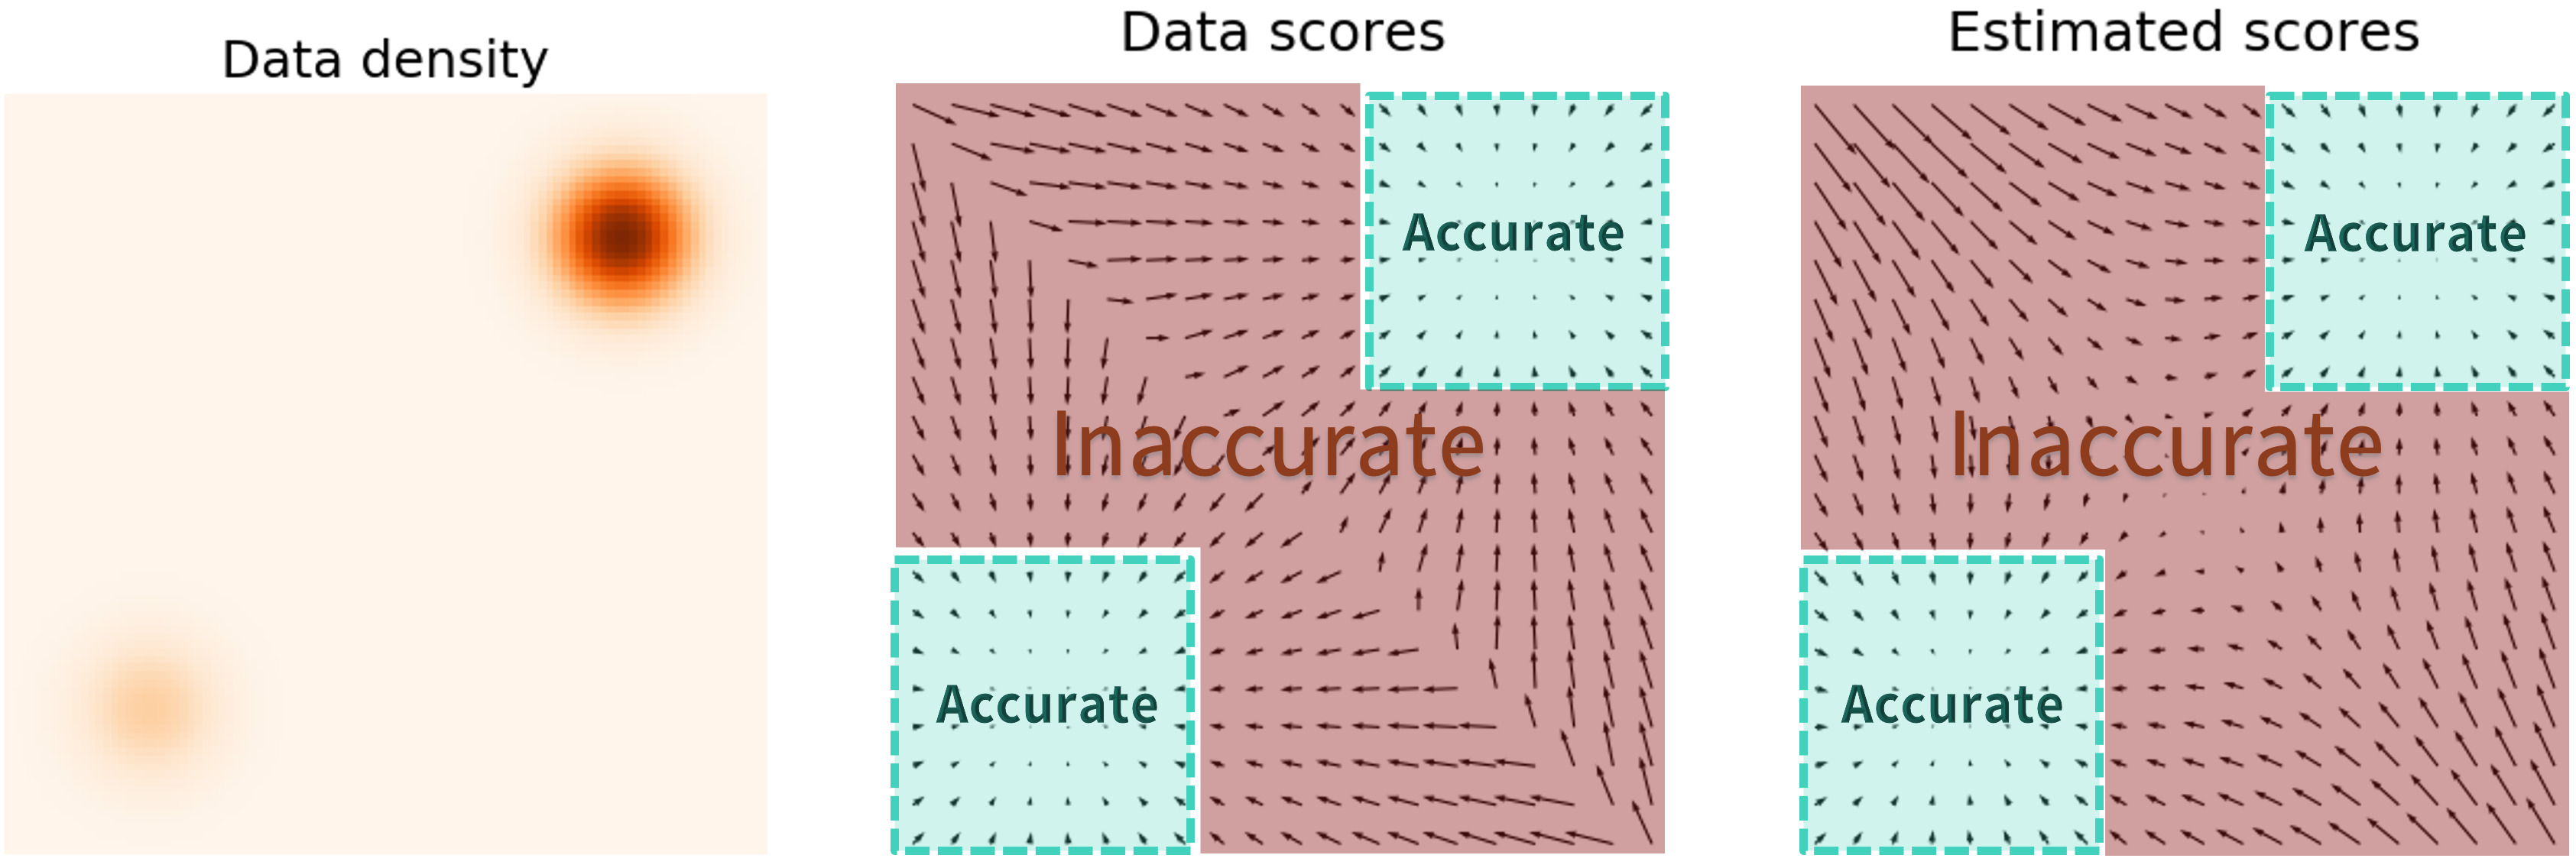
\includegraphics[width=0.8\linewidth]{gfx/low_density_probs.png}
    \caption{Score estimation for low density regions in the case of Gaussian mixtures. Source : \url{https://yang-song.net/blog/2021/score/}}
    \label{fig:low_d_estimation}
\end{figure}
This raises the following question : \textbf{How can one account for accurate estimation of the score in low density regions ?}
\subsection{Injecting more noise}
In order to account for accurately estimating the score for regions with low density, \citep{song2020generativemodelingestimatinggradients} propose to inject noise in several scales to the data points. When the noise scale $\sigma$ is sufficiently high, regions with low density for distribution $P$ are more likely to be populated for distribution $P_{\Sigma}$. This induces a trade-off between the magnitude of the added noise, i.e the size of $\sigma$, which populates the low density regions, and the alteration to the data distribution. In order to circumvent this issue, \citep{song2020generativemodelingestimatinggradients} propose \textit{annealed Langevin dynamics}, which consists in altering data with several noise scales $\sigma_{1},\sigma_{2},\ldots \sigma_{L}$, and training the model to minimize the following sum of score matching losses at different noise scales : 
\begin{equation}\label{eq:annealed_langevin}
    J_{ASM}(\theta) = \sum_{i=1}^{L} \lambda(i)E_{p_{\sigma_{i}}}\left[ ||\nabla \log p(x) - s_{\theta}(x,i)||^{2}  \right]
\end{equation}
where $\lambda(i)$ is a weighting schedule, and $s_{\theta}(x,i)$ is a model that takes in input the current point and the scale of the added noise. Note that the terms in equation \ref{eq:annealed_langevin} can be approximated using the aforementioned score matching techniques.
Once a model is trained to minimize $J_{ASM}$, the sampling procedure generating samples from $\hat{P}$ is described by algorithm \ref{algo:ald}.
\begin{algorithm}
\caption{Annealed Langevin Dynamics for Sampling \citep{song2020generativemodelingestimatinggradients}}
\begin{algorithmic}[1]\label{algo:ald}
\Require{Sequence of noise levels $\{\sigma_i\}_{i=1}^L$, step size $\epsilon$, number of iterations $T$}
\State Initialize $x_0$
\For{$i \leftarrow 1$ to $L$}
    \State Set step size $\alpha_i \leftarrow \epsilon \cdot \frac{\sigma_i^2}{\sigma_L^2}$
    \For{$t \leftarrow 1$ to $T$}
        \State Draw $z_t \sim \mathcal{N}(0, I)$
        \State Update $x_t \leftarrow x_{t-1} + \frac{\alpha_i}{2} s_\theta(x_{t-1}, \sigma_i) + \sqrt{\alpha_i} z_t$
    \EndFor
    \State Set $x_0 \leftarrow x_T$
\EndFor
\State \textbf{return} $x_T$
\end{algorithmic}
\end{algorithm}
\citep{sohldickstein2015deepunsupervisedlearningusing,ho2020denoisingdiffusionprobabilisticmodels} proposed a similar framework that was labeled as \textit{denoising diffusion probabilistic models}. Akin to \citep{song2020generativemodelingestimatinggradients}, they propose a noise scale $\beta{1},\beta{2},\ldots,\beta_{L}$, and they create a Markov chain for each training point $x_{0} \rightarrow \{x_{0},x_{1},\ldots,x_{L}\}$, where each $x_{i} \sim \mathcal{N}(\sqrt{1-\beta_{i}}x_{i-1},\beta_{i}I_{d})$, thus $x_{i} \sim \mathcal{N}(\sqrt{\alpha_{i}}x_{0},(1-\alpha_{i})I_{d})$, with $\alpha_{i} = \prod_{k=1}^{i}(1-\beta_{k})$. By denoting $p(x_{i}|x_{0}) = \mathcal{N}(x_{i}|\sqrt{\alpha_{i}}x_{0},(1-\alpha_{i})I_{d})$, a noise conditional model $s_{\theta}(\Tilde{x},i)$ is trained to minimize the following objective, that is similar to the one described by equation \ref{eq:annealed_langevin} : 
\begin{equation}\label{eq:ddpm}
    \mathcal{J}_{DDPM}(\theta) = \sum_{i=1}^{L} (1-\alpha_{i})\mathbb{E}_{p} \left[ \mathbb{E}_{p(.|x)}\left[ ||s_{\theta}(\Tilde{x},i) - \nabla \log p(x_{i}|x)||^{2} \right]  \right]
\end{equation}
The sampling process is done by starting from $x_{L} \sim \mathcal{N}(0,I_{d})$, then reversing the Markov chain :
\begin{equation}
    x_{i-1} = \frac{1}{1-\beta_i} \left( x_i + \beta_i s_\theta(x_i, i) \right) + \sqrt{\beta_i} z_i
\end{equation}
with $z_{i} \sim \mathcal{N}(0,I_{d})$ and $i \in \{L,\ldots,1\}$.
The generative procedure described by \citep{ho2020denoisingdiffusionprobabilisticmodels} is an alternative to using Langevin dynamics for generating samples using an estimated score, but one sees numerous similarities with the method proposed by \citep{song2020generativemodelingestimatinggradients}. Notably, both methods use increasing noise schedules to perturb the points, and estimate a noise conditional score model. One can thus ask : \textbf{Is there a unifying framework for generating with noise conditional score models ?}
\subsection{Diffusion process}
The answer to this question was obtained by answering another question : What happens when $L \rightarrow \infty $, i.e when the number of noise scales is infinite ? 
\\
When $L \rightarrow \infty$, the number of perturbations can be viewed as continuous and increasing noise perturbations. Thus, this can be seen as a stochastic process, and can sometimes be the solution of stochastic differential equations (SDEs). In order to generalize the idea of denoising score matching to continuous noise injections, we can mention diffusion processes. 
Diffusion processes are derived from modeling the dynamics of molecular systems, particularly from the theory of Langevin dynamics. In summary, a simplified model of a system can be created by compensating the omitted degrees of freedom through stochastic differential equations.
Fundamentally, a diffusion process $\{x_{t}\}_{t=0}^{T}$ is a Markov process indexed by a continuous time variable $t \in [0,T]$. By adding iteratively  noise to the samples, one can describe the \textit{forward} diffusion process as a solution the following Itô SDE : 
\begin{equation}\label{eq:forward_diff}
    dx = f(x,t)dt + g(t)dw 
\end{equation}
where dw is the standard Wiener process (Brownian motion). $f(x,t)$ is called the \textit{drift} coefficient of $x(t)$ and $g(t)$ is called the \textit{diffusion} coefficient of $x(t)$. The distribution of $x_{T}$  when $T \rightarrow \infty$ is called the \textit{prior} distribution and can be carefully chosen by tailoring $f$ and $g$ in the aforementioned SDE \citep{song2021scorebasedgenerativemodelingstochastic}.
Equation \ref{eq:forward_diff} has a unique solution when the drift and diffusion coefficients are Lipschitz in all of their arguments \citep{oksendal2003stochastic}. Generally, one chooses $f$ and $g$ such that $p_{T}$ is an easy distribution to sample from, like a zero-mean isotropic Gaussian distribution. 
For instance, with a linear drift $f(x) = -x$ and a constant diffusion coefficient $g(t) = \sqrt{2}$, one has that $p_{T}$ converges exponentially fast to $\mathcal{N}(0,I_{d})$ (CITATION).
In the following, we denote $P_{t}$ as the distribution of a sample from $P$ at timestep $t$. We also denote by $p_{t}(x_{t}|x_{0})$ the conditonal distribution of a noisy point $x_{t}$ after starting with point $x_{0}$.
When does the score intervene in this case ? \citep{ANDERSON1982313} proves that the reverse of a diffusion process, starting at distribution $P_{T}$ and ending in distribution $P$ is also a diffusion process, solution to the following SDE, that we label as the \textit{backward SDE} : 
\begin{equation}\label{eq:backward_diffusion}
    dx = \left(f(x,t) - g(t)^{2}\nabla \log p_{t}(x)dt\right) + g(t)dw
\end{equation}
Thus, if one learns $\nabla \log p_{t}(x)$ for $t \in [0,T]$, one can sample from $P$ by first sampling a point from $P_{T}$ and solving equation \ref{eq:backward_diffusion}.
\citep{song2021scorebasedgenerativemodelingstochastic} propose thus a continuous version of the discrete noise conditional score estimation, with the following objective function : 
\begin{equation}
    J_{\text{CSM}}(\theta) =\mathbb{E}_{t} \left[ \lambda(t) \mathbb{E}_{P} \left[ \mathbb{E}_{P_{t}} \frac{1}{2} \left\| s_{\theta}(x_{t},t) - \nabla_\mathbf{x} \log p_{t}(x_{t}|x) \right\|^2 \right]\right]
\end{equation}
Once the score is accurately estimated, one can solve the backward SDE using $s_{\theta}(x,t)$ as an estimator for $\nabla \log p_{t}(x)$. Several solving schemes are available, notably numerical solvers that discretize the backward SDE such as the stochastic Runge-Kutta and Euler-Maruyama methods \citep{kpj1992numerical}. Algorithm \ref{algo:sample_diffusion} describes this sampling procedure using the Euler Maruyama sampler. Furthermore, \citep{song2021scorebasedgenerativemodelingstochastic} proposed a different sampling method by using the corresponding deterministic reverse process, labeled as the \textit{probability flow} ordinary differential equation (ODE). It is expressed as : 
\begin{equation}\label{eq:backwatd_ode}
    dx = f(x,t) - \frac{1}{2}g(t)^{2}\nabla \log p_{t}(x)dt
\end{equation}
and can be equivalently solved by ODE numerical solvers that discretize the ODE. This version provides a computational advantage as less discretization steps are needed for a fair quality, but there is a tradeoff between image quality by SDE generation and the number of function evaluations (computation cost) via ODE generation \citep{xu_restart_2023}. 

\begin{multicols}{2}

\begin{algorithm}[H]
\caption{Training a Score-based Diffusion Model}
\begin{algorithmic}[1]\label{algo:train_diffusion}
\Require{Dataset $\mathcal{D}$, learning rate $\eta$}
\State Initialize parameters $\theta$
\While{not converged}
    \State Sample mini-batch $\{x^{(i)}\}$ from $\mathcal{D}$
    \State Update $\theta \gets \theta - \eta \nabla_\theta \mathcal{J}_{CSM}(\theta)$
\EndWhile
\State \Return{Trained model parameters $\theta$}
\end{algorithmic}
\end{algorithm}

\columnbreak

\begin{algorithm}[H]
\caption{Sampling via Discretized Backward SDE}
\begin{algorithmic}[1]\label{algo:sample_diffusion}
\Require{Trained parameters $\theta$, number of steps $N$, time horizon $T$}
\State Initialize $x_T \sim p_T(x)$ (e.g., Gaussian)
\State Initialize current timestep $t_{n} = T$
\For{$n = N$ down to $1$}
    \State Set time step $\Delta t = T / N$
    \State Update current timestep $t_{n} = t_{n} - \Delta t$
    \State Sample noise $\epsilon_n \sim \mathcal{N}(0, I)$
    \State Update using backward SDE discretization:
    \[
    x_{n-1} = x_n - s_\theta(x_n, t_n) \Delta t + \sqrt{\Delta t} \epsilon_n
    \]
\EndFor
\State \Return{Sample $x_0$}
\end{algorithmic}
\end{algorithm}

\end{multicols}
\citep{karras2022elucidatingdesignspacediffusionbased} proposed a unifying framework for diffusion-based generative models, and showed that different sampling schemes can be used with the same diffusion model. 
Table \ref{tab:diffusion_table} lists a few configurations for popular diffusion based generative models. 

\begin{table}[ht]
\centering
\caption{Specific design choices employed by different model families}
\begin{tabular}{@{}m{1.5cm}m{4cm}m{4cm}m{4cm}@{}}\label{tab:diffusion_table}
\toprule
\textbf{Model} & \textbf{VP} \citep{song2020generativemodelingestimatinggradients} & \textbf{VE} \citep{ho2020denoisingdiffusionprobabilisticmodels} & \textbf{EDM \citep{karras2022elucidatingdesignspacediffusionbased}} \\
\midrule
\textbf{ODE Sampling} & Euler & Euler & 2nd order Heun \\
\textbf{Time steps $t_i$} & $1+\frac{i(1-\epsilon_{0})}{N-1}$ & $\sigma^{2}_{max}\left(\frac{\sigma_{min}^2}{\sigma_{max}^2}\right)^{\frac{i}{N-1}}$ & $t$ \\
\midrule
\textbf{Training (Sec. 5)} & & & \\
\textbf{Noise distribution} & $\sigma^{-1}(\sigma) \sim \mathcal{U}(\epsilon_{t},1)$ & $\ln(\sigma) \sim \mathcal{U}(\ln(\sigma_{min}), \ln(\sigma_{max}))$ & $\ln(\sigma) \sim \mathcal{N}(P_{mean}, P_{std}^2)$ \\
\textbf{Loss weighting $\lambda(\sigma)$} & $\frac{1}{\sigma^2}$ & $\frac{1}{\sigma^2}$ & $\left(\frac{\sigma^2 + \sigma^2_{data}}{\sigma \cdot \sigma_{data}}\right)^2$ \\
\bottomrule
\end{tabular}
\end{table}
Thus, diffusion appears as a viable choice for approximating probability distributions. However, as most distribution approximation methods, estimation errors arise in practice. For the diffusion framework, there is two main sources of error : \textbf{approximation} errors related to the training of the score, and \textbf{sampling} errors related to the discretization of the backward ODE or SDE. \citep{lai2023fpdiffusionimprovingscorebaseddiffusion,chao2023investigatingconservativepropertyscorebased} notably showed that diffusion models in practice are not conservative for large values of $t$, i.e does not define vector fields of real valued functions.
This poses a new challenge, which is to mitigate the error sources related to estimation. As generation consists of both training and sampling, this calls for improvement during both the training and the sampling stages. Thus, we ask the following question : \textbf{How to refine the generative process ?} In the following section, we will answer this broadly for generative models and specifically provide an answer for diffusion models in sections \ref{sec:dg} and \ref{sec:rl}.
By noting $\Tilde{P}$ the distribution induced by training a generic generative model and sampling from it, one can check a discrepancy measure between the two distributions (Definition \ref{def:divergence}) to evaluate \textit{how accurate} the estimation procedure is. In our work, we will focus on the family of f-divergences, that compute the following metric with respect to the Lebesgue measure : 
\begin{equation}
    D_{f}(\Tilde{P}||P) = E_{P}\left[f(\frac{P}{Q})\right] = \int p(x)f(\frac{p(x)}{\Tilde{p}(x)}dx
\end{equation}
\section{Expressivity of a generative model}
\label{sec:related:improve_generation}
The sources of error of interest in our case are the expressivity of the considered model, and the stopping iteration. When the number of iterations goes to infinity, the expressiveness of the family of parameters yield an optimal distribution $\Tilde{P}$ for a given f-divergence, that is not necessarily equal to $P$. One controls the expressivity of a model by architecture design, choice of the objective function, and training paradigm. 
\subsection{Precision and recall as f-divergences}\label{subsec:precision_recall}
For generative models in general, the choice of an $f$ in the minimization of an $f$-divergence yields different results in practice, for the same family of models. For instance, \citep{minka2005divergence} observed that optimizing Kullback-Leibler divergence( $f(x) = x \log x$) tends to favor \textit{mass-covering} models and that optimizing the reverse KL ($f(x) = -\log x$) and Jensen-Shannon $f(x) = \frac{1}{2}\left( x\log x - (x+1)\log \left( \frac{x+1}{2} \right) \right)$
tends to favor \textit{mode-seeking} behaviors. Here, a mass covering model will produce diverse samples, covering a substantial part of the support of $P$. Conversely, a mode seeking model will display less diversity in the produced samples, but the generated samples will have a high target density $p$, which make them more \textit{precise}.
Depending on the use case, one would either want to produce samples of high quality or with high diversity. For example, using generative models for drug discovery would require precise samples, while using them to generate images for artistic synthesis might allow less precision for more diversity. INSERT PLOT HERE LIKE FIGURE 4.3 from alex thesis. This implicit trade-off was investigated by \citep{verine2024precision} in the context of GANs and normalizing flows, and they derive a new divergence, termed as the precision and recall (P\&R) divergence, that is dependent on a specified trade-off parameter $\lambda$. It is essentially an $f$-divergence, with a function $f_{\lambda}$ defined as : 
\begin{equation}
  f_{\lambda}(x) =
  \begin{cases} 
    \max(\lambda x,1) - \max(\lambda,1) & \text{if } \lambda \in [0,+\infty[ \\
    \mathbf{1}_{x=0} & \text{if } \lambda = +\infty.
  \end{cases}
\end{equation}
In order to control the expressivity of a generative model with a specified trade-off between diversity and precision, \citep{verine2024precision} propose a method for GANs and normalizing flows, that improves upon the traditional framework of $f$-GANs introduced by \citep{nowozin2016fgantraininggenerativeneural}.
Modifying the objective functions is thus a foundational method to control the expressivity of a generative model. This, in practice however, is not directly applicable to diffusion models as the loss is not expressed as an $f$-divergence, but rather as a score matching loss. In the following subsections, we will give examples that improve the expressivity of a score based model.


\subsection{Using the theory of diffusion as a refinement process}
We will give two examples that improved the likelihood of the generated distribution of diffusion models. One is based on conservativity, a fundamental property that the estimated score should satisfy, and another is based on the FOkker-Planck equation, that is related to the SDE formulation of score based models.
\begin{definition}
    A vector field, represented by a \textit{vector} valued function $v : \mathcal{X} \rightarrow \mathbb{R}^{d}$, is said to be conservative if it can be expressed as the gradient of a real valued function
\end{definition}
By definition, the ground truth score $s(x,t) = \nabla_{x} \log p_{t}(x)$ is thus conservative. However, \citep{salimans2021should,chao2023investigatingconservativepropertyscorebased} highlighted that notable diffusion models, that are defined as U-Nets in practice, are not conservative. In order to ensure conservativity, \citep{salimans2021should,saremi2018deepenergyestimatornetworks} propose to constrain the architecrure of the model such that its output vector field is modeled as a gradient of a real valued function. This, however, constrains the expressivity of the architecture overall. \citep{chao2023investigatingconservativepropertyscorebased}, on the other hand, add a regularization term based on higher orders of the score to ensure the conservativity. This method allowed for more flexible architecture choices, and an improvement in likelihood computations of the estimated distributions. We will now present another method that helped enforce conservativity, introduced by \citep{lai_fp-diffusion_2023}.
The ground truth density $p_{t}$ associated to the forward diffusion SDE (equation \ref{eq:forward_diff}) satisfies the Fokker-Planck equation \citep{oksendal2003stochastic} : 
\begin{equation}\label{eq:fokker_plack}
  \frac{\partial p_t(x)}{\partial t} = -\frac{\partial}{\partial x} \left[ f(x, t) p_t(x) \right] + \frac{\partial^2}{\partial x^2} \left[g(t) p_t(x) \right]
\end{equation}
\citep{lai_fp-diffusion_2023} derive from this equation another equation that the ground truth score should satisfy, labeled as \textbf{the score FPE} (c.f Proposition 3.1 and Appendix G in \citep{lai_fp-diffusion_2023}) : 
\begin{equation}\label{eq:score_fpe}
    \frac{\partial s(x,t)}{\partial t} = \nabla_{x}\left[\frac{1}{2}g^{2}(t)\mathrm{div}_{x}(s(x,t)) + \frac{1}{2}g^{2}(t)\left|\left|s(x,t)\right|\right|^{2} - \langle f(x,t),s(x,t) \rangle - \mathrm{div}_{x}(f(x,t))\right]
\end{equation}
where $s(x,t) = \nabla_{x} \log p_{t}(x)$ denotes the ground truth score, and $\mathrm{div}_{x}(s(x,t))= \sum_{i=1}^{d}\frac{\partial s(x,t)}{\partial x_{i}} $ denotes the divergence of the vector field $s(x,t)$. In practice, it is observed that most trained diffusion models do not satisfy the score FPE. By denoting by $\mathcal{R}(.) $ as the linear mapping corresponding to the right hand side of equation \ref{eq:score_fpe}, one can define a \textit{residual} $\epsilon_{\theta}$ corresponding to the difference $\frac{\partial s_{\theta}(x_{t},t)}{\partial t} - \mathcal{R}[s_{\theta}](x_{t},t) $, evaluating how far the current estimated score is from satisfying the score FPE. This residual is added as a regularization term in various forms, depending on the used score matching loss, and thus enforces the score FPE to be satisfied.
\citep{lai_fp-diffusion_2023} demonstrate that notable implications of satisfying equation \ref{eq:score_fpe} are : 
\begin{itemize}
    \item Reducing the KL divergence between the target distribution $P_{0}$ and the estimated density with ODE sampling (solved by discretization of equation \ref{eq:backwatd_ode})
    \item Enforcing the conservativity of the vector field $s_{\theta}(x_{t},t)$
\end{itemize}
These methods elaborate a novel framework that is suitable for a more theoretically grounded training for diffusion based models. One of the immediate setbacks of adopting these methods is their incompatibility with pre trained models, that already display a good performance. We thus ask : \textbf{Are there methods that improve the generative process without retraining a model from scratch ? cCan they be used for a wide array of models ?}
\subsection{Fine-tuning methods}
\citep{lucic2019highfidelityimagegenerationfewer} first noticed that when a GAN is generating data in a label limited setting, there was a significant advantage in using class labels during generation. Using this idea, \citep{dhariwal2021diffusionmodelsbeatgans} presents a boosting method for diffusion models, by incorporating class-specific information during the sampling process through a classifier. This idea was presented in order to make diffusion models increase their precision at the expense of their diversity (c.f subsection \ref{subsec:precision_recall}.
Specifically, given a specified class $y$, one can train a classifier with a parameterized model $c_{\phi}$ to estimate $\nabla \log p(y|x_{t},t)$ for every perturbed point $x_{t}$ at every diffusion step $t$. Then, the sampling transition is done by replacing $p(x_{t}|x_{t+1})$ by $p(x_{t}|y,x_{t+1})$, i.e the score approximation becomes $s_{\theta}(x_{t},t) + \lambda c_{\phi}(x_{t},t,y)$, where $\lambda$ is a scaling parameter that determines the influence of classifier guidance. This technique is not involved in the training of the diffusion model, and can be used as a \textit{refinement} method for fine-tuning the diffusion model. Notably, it can present advantages in terms of computational resources, as a smaller model can be used as a classifier. We will be exploring another boosting method, namely discriminator guidance, as a main improvement framework for diffusion models in chapter \ref{sec:dg}.


\fbox{\parbox{\linewidth}{\textbf{Note :} This method was further extended by \citep{ho2022classifierfreediffusionguidance} to \textit{classifier-free} guidance, by simultaneously training a model on samples x and a context $c$. This is a boosting-free method as only the training procedure is affected, and no additional model is trained. Stable diffusion \citep{rombach2022highresolutionimagesynthesislatent}, among others, used this method during its training, which explains its ability to generate data from user defined prompts.
Adding context information is thus a viable technique to improve the generative process. }}
\\
Another family of methods consists in using statistical sampling algorithms to improve the likelihood of a sample. In the following, we will describe rejection algorithms for generative models, as they rely on density ratio estimation techniques that will be important for the following chapters, notably chapters \ref{sec:dg} and \ref{sec:rl}. 
Rejection sampling \citep{vonN51} is a method for sampling from a target distribution $P$ using a proposal distribution $Q$ and a density ratio $\frac{p(x)}{q(x)}$ between both distributions. In the context of generative models, the idea is to create a new distribution $\Hat{P}$ from the estimated distribution $\Tilde{P}$ by using accepting or rejecting samples from $\Tilde{P}$ with a rejection probability $a(x)$. The resulting density is given by $\hat{p}_{a}(x) = \frac{\Tilde{p}(x)a(x)}{Z}$, where $Z$ is a normalization constant. Thus, the rejection rate is given by $\mathbb{E}_{\Tilde{P}}[a(x)] = \frac{1}{Z}$ or in other terms, one needs to draw $\frac{1}{Z}$ samples in average from $\Tilde{P}$ to have one sample accepted.
\begin{algorithm}
\caption{Generic Rejection Sampling Algorithm}
\begin{algorithmic}[1] % The number tells where the line numbering should start
\State Generate $x \sim \Tilde{P}$
\State Generate $u \sim \mathcal{U}(0,1)$
\While{$u \leq a(x)$} \Comment{Rejection criterium}
    \State $x \sim \Tilde{P}$
    \State $u \sim \mathcal{U}(0, 1)$ \Comment{Draw a uniform random number}
\EndWhile
\end{algorithmic}
\end{algorithm}
In order to exactly match the target density $p(x)$, the literature has proposed an optimal rejection rate $a(x)$ of the form : 
\begin{equation}\label{eq:optimal_rejection}
    a_{\mathrm{opt}}(x) = \frac{p(x)}{M\Tilde{p(x)}}
\end{equation}
where $M = \sup_{\mathcal{X}} \frac{p(x)}{\Tilde{p(x)}}$ and the resulting density function of $\Hat{P}_{a_{\mathrm{opt}}}$ is equal to $p$. However, in a high dimensional $\mathcal{X}$, \citep{mackay2003information} showed that $M$ can be very high and thus set a high rejection rate. For example, in the context of BigGAN \citep{brock2019largescalegantraining} trained on the CelebA dataset \citep{liu2015faceattributes} (178×218 images), the rejection rate is as big as $10^{6}$. Thus, a line of work investigates alternative rejection probabilities $a(x)$ to perform rejection sampling in high dimensions.
\\
In the context of GANs, \citep{azadi2019discriminatorrejectionsampling} propose to involve the discriminator in the \textit{generation} process by using it to estimate the density ratio involved in equation \ref{eq:optimal_rejection}. A discriminator model $d$ parameterized by a set of parameters $\phi$ within the framework of $f$-GANs (\citep{nowozin2016fgantraininggenerativeneural},\ref{eq:f_gan}) can be used to estimate the density ratio using the following expression \citep{verine2024precision}: 
\begin{equation}\label{eq:discriminator_density_ratio}
    \frac{p(x)}{\Hat{p}(x)} \approx \nabla f^{*}(d_{\phi}(x)) = r(x)
\end{equation}
where $f^{*}$ denotes the \textit{Fenchel conjugate} of function $f$. In order to lower the rejection rate, \citep{azadi2019discriminatorrejectionsampling} propose to use the following acceptance probability function : 
\begin{equation}\label{eq:acceptance_bounded}
    a_{\gamma}(x) = \frac{r(x)}{r(x)(1-e^{\gamma}) + e^{\gamma}M}
\end{equation}
Negative values of $\gamma$ are used to lower the rejection rate, but no theoretical contributions are given for the choice of $\gamma$. 
Another line of work explores rejection sampling methods under a \textit{budget}. That is, under budget $K$, solve the following optimization problem : 
\begin{align*}\label{eq:budget_rejection_prob}
\min_a \quad & D_f(P \parallel \tilde{P}_a) \\
\text{s.t.} \quad & 
\begin{cases} 
\mathbb{E}_{\hat{P}}[a(x)] \geq \frac{1}{K}, \\
\forall x \in X, \quad 0 \leq a(x) \leq 1.
\end{cases}
\end{align*}
\citep{verine2024optimalbudgetedrejectionsampling} derives an optimal solution for this problem, with a rejection probability of the form : 
\begin{equation}
    a_{\mathrm{K-opt}}(x) = \min \left(\frac{p(x)c_{K}}{\tilde{p(x)}M},1\right)
\end{equation}
where $c_K$ is a constant such that $\mathbb{E}_{\Tilde{P}}[a_{\mathrm{K-opt}}(x)] = \frac{1}{K}$
The density ratio ratio is computed by a discriminator as in \citep{azadi2019discriminatorrejectionsampling}, and the constant $c_{K}$ is computed using dichotomy.

\section{Conclusion}
Diffusion models emerge as a viable family of generative models, as they emanate from a nice theoretical framework. The generation process is two-folds : training a model $s_{\theta}$ to estimate the target score function at each noise level $t in [0,T]$, then use the estimated score to solve the backward SDE (Equation \ref{eq:backward_diffusion}) or ODE (Equation \ref{eq:backwatd_ode}). While this separation allows for separately improving each step of the process, it might represent a concatenation of two error sources : an approximation error related to the training process, and an estimation error related to the sampling process.
Several diffusion models are currently state of the art in generation, and the main question of our work is how to improve these pre-trained models, without retraining them and without additional data. In subsection \ref{sec:diffusion}

This raises the following questions, that we will try to answer in chapter \ref{sec:related:improve_generation}, we presented a few ideas to improve generative models, and booting methods emerged as a viable technique to do so. This raises the following question : 
\begin{itemize}
    \item \textbf{Can classifier guidance be generalized to a boosting method that does not rely on class information ?} This question is answered in chapter \ref{sec:dg}, where we introduce discriminator guidance \citep{kim2023refininggenerativeprocessdiscriminator} and improve the theoretical framework of this method.
    \item \textbf{Can we extract further information from the density ratio estimated by a discriminator ?} This question will be answered in chapter \ref{sec:rl}, where we introduce reinforcement learning methods that uses information from an estimated density ratio as a reward function. 
\end{itemize}
\label{sec:related:conclusion}


 % INCLUDE: related work
% !TEX root = ../thesis-example.tex
%
\chapter{Discriminator guidance}\label{sec:dg}

How to improve the generation process of a diffusion model without re-training it ? In this chapter, we will present discriminator guidance, a concept introduced by \citep{kim2023refininggenerativeprocessdiscriminator} and improved in the context of this master's thesis. Overall, this method consists in using information from a trained discriminator during the sampling process, to guide the denoising path towards the target distribution. This can be seen as a generalization of classifier guidance \citep{dhariwal2021diffusionmodelsbeatgans} to the case of the absence of class information, and can also linked to discriminator rejection \citep{azadi2019discriminatorrejectionsampling} if applied to diffusion models.
We will first start by presenting the framework proposed by \citep{kim2023refininggenerativeprocessdiscriminator} in section \ref{sec:dg:sec1}, The formulation of this framework is theoretically grounded, but the presented training scheme of the discriminator is not justified. We show in section \ref{sec:dg:sec2} that it is sub-optimal, and can worsen the sampling process in the over-fitting regime. Thus, in section \ref{sec:dg:sec3}, we propose a novel training objective that is optimal and demonstrate our results for standard generation benchmarks.
\\
In the following, we recall the notation used in our work :
\begin{itemize}
    \item $P_{t},p_{t}$ denotes the diffused \textit{target} distribution and its corresponding density at time $t$
    \item $s_{\theta}(x,t)$ denotes a \textbf{trained} score based model with fixed parameter set $\theta$
    \item $\Tilde{P}_{t},\Tilde{p}_{t}$ denotes the diffused \textit{estimated} distribution and its corresponding density at time $t$ obtained by solving \textit{exactly} the backward SDE (\ref{eq:backward_diffusion}). We assume that $s_{\theta}(x,t) = \nabla_{x}\log\Tilde{p}_{t}(x)$
    \item The trainable discriminator $d_{\phi}$ is parameterized by a set of parameters $\phi$
    \item We denote by $\pi(x)$ the density of the prior distribution used in the sampling process.
    \item The \textit{refined} distribution induced by using both the score network $s_{\theta}$ and a discriminator $d_{\phi}$ is denoted by $\Hat{P}_{t}$ and its corresponding density by $\Hat{p}_{t}$
\end{itemize}

\section{Discriminator guidance}\label{sec:dg:sec1}
\subsection{Derivation}
Discriminator guidance stems from the simple concept of estimating the training error $\nabla \log p_{t}(x) - s_{\theta}(x,t)$.
In the following, we provide a definition that would introduce a key assumption in the derivation of discriminator guidance.
\begin{definition}
    The evidence lower bound $\mathcal{L}_{\theta}$ of a score model $s_{\theta}$ is given by :
    \begin{equation}
            \mathcal{L}(s_{\theta}) = \frac{1}{2}\int_{0}^{T} \lambda(t) \mathbb{E}_{P}\left[||\nabla \log p_{t}(x) - s_{\theta}(x,t) ||^{2}  \right]dt
    \end{equation}
\end{definition}


In the following, we make the following assumption : 
\begin{assumption}\label{ass:elbo}
    The distribution  $\Tilde{P}_{t}$ induced by the backward process with score estimator $s_{\theta}$ has a log likelihood equal to the evidence lower bound of $s_{\theta}$
\end{assumption}
Define $S_{\mathrm{sol}}$ to be a family of time-conditioned score network $s_{\theta}$ that satisfies the
following: there exists densities $p_{\theta,0}$ and $p_{\theta,t}$ such that$ s_{\theta}(x, t) = \nabla log p_{\theta,t}(x)$ almost everywhere, where $p_{\theta,t}$ is the marginal density at time t of $dx = f(x, t) dt + g(t) dw$, starting from $x_{0} \sim p_{\theta,0}$
\begin{theorem}\label{thm:conservativity_score}\citep{kim2023refininggenerativeprocessdiscriminator}
    Suppose that the score network $s_{\theta}$ satisfies assumption \ref{ass:elbo}. Then $s_{\theta} \in S_{\mathrm{sol}}$. We thus denote by $\Tilde{P}_{t}$ the distribution with density $\Tilde{p}_{t}(x)$ such that $s_{\theta}(x,t) = \nabla \log \Tilde{p}_{t}(x)$
\end{theorem}



\begin{theorem}\label{theorem:dg_sde}\citep{kim2023refininggenerativeprocessdiscriminator}
Suppose that :
\begin{itemize}
    \item Assumption \ref{ass:elbo} is satisfied by the estimated score network $s_{\theta}$.
    \item  $s_{\theta}(x,T) = \nabla \log \pi(x)$.
\end{itemize}
Then, by noting $c_{\theta}(x,t) = \nabla \log p_{t}(x) - s_{\theta}(x,t) = \nabla \log \frac{p_{t}(x)}{s_{\theta}(x,t)}$, the backward SDE defined by : 
\begin{equation}\label{eq:refined_backward_SDE}
    dx = f(x,t) - \frac{1}{2}g(t)^{2}(s_{\theta}(x,t) + c_{\theta}(x,t))dt
\end{equation}
coincides with the backward SDE of the diffusion process induced by the target distribution (Equation \ref{eq:backward_diffusion}).  
\end{theorem}
The proofs for theorems \ref{thm:conservativity_score},\ref{theorem:dg_sde} are relegated to Appendix \ref{sec:appendix}.\\
Thus, if one estimates exactly the density ratio $r_{\mathrm{opt}}(x,t) = \frac{p_{t}(x)}{\Tilde{p}_{t}(x)}$, then the \textit{refined} score $s_{\theta,\mathrm{opt}}(x,t) = s_{\theta}(x,t) + \nabla \log r_{\mathrm{opt}}(x,t)$ allows for sampling from the target distribution by solving the backward SDE. \citep{kim2023refininggenerativeprocessdiscriminator} train a discriminator $d_{\phi}(x,t)$ to estimate $r_{\mathrm{opt}}(x,t)$ then computes $\nabla \log d_{\phi}$ as an estimator for $c_{\theta}$. This raises the following question : \textbf{Does a generic estimation of the density ratio make the generative process better ?}
\subsection{f-divergence between the target and refined distribution}
The following theorem follows from the conservativity of $s_{\theta}$ (Assumption \ref{ass:conservativity_refined}) : 
\begin{theorem}\label{ass:conservativity_refined}
    Suppose that the assumptions of theorem \ref{theorem:dg_sde} are satisfied. The backward SDE using as a score estimator $s_{\theta,\phi}(x,t) = s_{\theta}(x,t) + \nabla \log d_{\phi}(x,t)$ induces a distribution $\Hat{P}_{t}$ with density $\Hat{p}_{t}(x)$
\end{theorem}
\citep{kim2022maximumlikelihoodtrainingimplicit} provide an interesting result that upper bounds the Kullback-Leibler divergence between the target and refined distributions.
\begin{theorem}\label{theorem:kl_refined}\citep{kim2023refininggenerativeprocessdiscriminator}
    If the assumptions of theorem \ref{theorem:dg_sde} hold, then given the target distribution $P_{t}$, the score distribution $\Tilde{P}_{t}$ and the refined distribution $\Hat{P}_t$ we have : 
    \begin{align*}
        D_{KL}(p_{0} \| \Tilde{p}_{0}) &= D_{KL}(p_{T} \| \pi) + E_{\theta}, \\
        D_{KL}(p_{0} \| \Hat{p}_{0}) &\leq D_{KL}(p_{T} \| \pi) + E_{\phi}
    \end{align*}
    \textit{where $E_{\theta}$ is the score error}
    \[
    E_{\theta} = \frac{1}{2} \int_0^T g^2(t) \mathbb{E}_{p_{t}} \left[ \|\nabla \log p_{t}(x) - s_{\theta}(x,t)\|^2 \right] dt,
    \]
    
    \textit{and $E_{\phi}$ is the discriminator-adjusted score error}
    
    \[
    E_{\phi} = \frac{1}{2} \int_0^T g^2(t) \mathbb{E}_{p_{t}} \left[ \|\nabla \log r_{\mathrm{opt}} - \nabla \log d_{\phi}\|^2 \right] dt.
    \]
    Leading to the following inequality : 
    \begin{equation}\label{eq:gain_inequality}
        D_{KL}(p_{0},\Hat{p}_{0}) \leq D_{KL}(p_{0},\Tilde{p}_{0}) + (E_{\theta} - E_{\phi})
    \end{equation}
\end{theorem}
\citep{kim2023refininggenerativeprocessdiscriminator} provides no theoretical analysis on the positivity of the difference $ (E_{\theta} - E_{\phi})$, but argue that in practice it is initialized near 0 and gradually increases throughout training.
Table \ref{tab:dg_gain} shows the value of the difference with different initializations of the discriminator. Notably, a completely blind discriminator $d_{\phi}(x,t) = \frac{1}{2}$ has $E_{\phi} = E_{\theta}$, and an optimal discriminator has zero error. 
 \begin{table}[ht]
\centering
\caption{Discriminator-adjusted score error $E_{\infty, \phi}$ and corresponding refinement value \citep{kim2023refininggenerativeprocessdiscriminator}.}
\label{tab:dg_gain}
\begin{tabular}{@{}lcc@{}}
\toprule
Discriminator        & $E_{\theta,\phi}$ & $ E_{\theta} - E_{\theta,\phi}$   \\ \midrule
Blind $d_{\phi} (t = 0.5)$ & $E_{\theta}$      & 0             \\
Optimal $d_{\phi}$  & 0                  & $E_{\theta}$ (Maximum) \\
Untrained $d_{\phi} (\approx 0.5)$ & $\approx E_{\theta}$ & $\approx 0$  \\
Trained $d_{\phi}$  & $\ll E_{\theta}$   & $\gg E_{\theta}$ \\ \bottomrule
\end{tabular}
\end{table}
There was however no analysis in the worst case scenario, where a discriminator is \textit{badly} trained. In section \ref{sec:dg:sec2}, we present situations that are possible in practice that could make the generation process worse.




\subsection{Training the discriminator}
In order to train the discriminator, \citep{kim2023refininggenerativeprocessdiscriminator} propose the same training paradigm as in GAN training. Specifically, a discriminator is trained to minimize the binary cross-entropy loss, as suggested in the seminal GAN paper by \citep{goodfellow2014generativeadversarialnetworks} : 
\begin{equation}\label{eq:bce}
    \mathcal{J}_{CE}(\phi) = \int_{0}^{T} \lambda(t) \mathbb{E}_{P_{t}}\left[-\log d_{\phi}(x,t) \right] + \mathbb{E}_{\Tilde{P}_{t}}\left[ -\log(1 - d_{\phi}(x,t))  \right]dt
\end{equation}
and the estimated density ratio is given by $r_{\phi}(x,t) = \frac{d_{\phi}(x,t)}{1 - d_{\phi}(x,t)}$. The corresponding correction term is thus given by $c_{\phi}(x,t) = \nabla \log r_{\phi}(x,t)$. 
Training is done by generating samples from the estimated score network to estimate the second expectation in equation \ref{eq:bce}, and samples from the dataset are used to estimate the first expectation in equation \ref{eq:bce}. The main advantage this loss is providing a relatively fast training time for the discriminator.
However, no theoretical analysis is provided regarding its ability to approximate $c_{\phi}(x,t)$, that is $\nabla \log r_{\mathrm{opt}}(x,t)$. Minimizing the cross entropy loss provides indeed a good estimate for the density ratio, but not necessarily for the gradient of the log density ratio.
\\
We thus raise the following question, that we answer in section \ref*{sec:dg:sec2} : \textbf{Even if the cross-entropy is minimized, is the discriminator guidance refining the diffusion model?}

\section{Sub-optimality of cross entropy minimization}\label{sec:dg:sec2}
In this section, we first show in theorem \ref{theorem:exploding_kl} that an arbitrarily low cross-entropy loss can lead to an arbitrarily high KL-divergence between the target and refined distribution. We then show in \ref*{theorem:expectation_exploding} that over-fitting the discriminator to minimize the cross-entropy leads to a high KL divergence between $P$ and $\Hat{P}$.



\begin{theorem}\label{theorem:exploding_kl}
    Let $\left\{\vx(t)\right\}_{t\in[0, T]}$ be a diffusion process defined by Equation~\ref{eq:forward_diff}. Assume that $\nabla \log \wtp_t= \vs_\theta$ and $\nabla \log \whp_t =\vs_\theta +\nabla \log r_\phi $ and that the induced distribution $P$, $\wtP$, and $\whP$ satisfies the assumptions detailed in Appendix~\ref{sec:appendix:assumptionssong}. Then, for every $\varepsilon>0$ and for every $\delta>0$, there exists a discriminator $\vd:\reals^d\times\reals\to\reals$ trained to minimize the cross-entropy such that:
    \begin{equation}
        \calL_{\mathrm{CE}}^{d}(\phi)\leq \varepsilon \et \KL(P\Vert \widetilde{P}) \geq \delta,
    \end{equation}
    where $\widehat{P}$ is the distribution induced by discriminator guidance with $\vd$.
\end{theorem}
\begin{hproof}The detailed proof for Theorem~\ref{theorem:exploding_kl} is provided in Appendix \ref{app:sec:proofsuboptimal}. The main idea for the proof is to show that a learned discriminator $d_{\phi}$ oscillating around the true optimal discriminator $d^*$ will show a low cross-entropy. The smaller the amplitude of the oscillation, the lower the cross-entropy. However, the faster the oscillations, the larger the Kullback-Leibler divergence will be. \end{hproof}
Although theorem \ref*{theorem:exploding_kl} shows the sub-optimality of the cross-entropy, it presents a pathologic case that one cannot find in practice. In the following theorem, we consider the situation where the discriminator overfits the training data, and show that the KL divergence between the target and refined distribution can explode.
\begin{theorem}\label{theorem:expectation_exploding}
    Let $P$ and $\widetilde{P}$ be two
distributions on $\mathbb{R}$. Assume the intersection of their support
is not empty, and assume they admit density functions $p$ and $\tilde{p}$
which are both $L$-Lipschitz. Let $x_{1}\ldots x_{N}\sim P^{N}$
and $x_{1}'\ldots x_{N}'\sim\tilde{P}^{N}$. Assume that the or cross-entropy loss $-\log\sigma\left(d_{\varphi}(x_{i})\right)$
and $-\log\left(1-\sigma\left(d_{\phi}(x'_{i})\right)\right)$
is at most $\epsilon$ on each example $x_{i}$ and $x_{i}'$. Then,
the expectation over the dataset of the mean square error exhibits
the following behavior, for some constant $c$:
\begin{equation}
    \lim_{N\rightarrow\infty}\frac{\mathbb{E}\left[E_{\phi}\right]}{N}\to c.
\end{equation}
In other words, the difference $E_{\theta} - E_{\phi}$  decreases linearly with the number of samples. This shows that the upper bound on the KL divergence between the target and refined distribution goes to $-\infty$ in an over-fitting regime.
\end{theorem}
\begin{hproof}The Theorem is proved in Appendix~\ref{sec:app:proofoverfitting}. While we assume a one-dimensional diffusion process for the sake of simplicity, this result could be applied to higher dimensional. The key argument is to show that if the discriminator is overfitting the cross-entropy, the values of $d_\phi$ on real and fake samples will be very different. However, the closer the distributions $P$ and $\whP$, the higher the probability of sampling a fake sample that is close to a real sample. Therefore, the discriminator gradient will be high between the two samples independently of the true gradient value.
\end{hproof}

Intuitively, these results are due to the fact that \citep{kim2023refininggenerativeprocessdiscriminator} provide a good estimation for the density ratio $\frac{p_{t}(x)}{\hat{p}_{t}(x)}$, but not for the gradient of the log density ratio.
This raises the following questions:
\begin{itemize}
    \item \textbf{How can we train the discriminator to provide a good estimate for the gradient of the log density ratio ?}
    \item \textbf{Instead of training a model to estimate the density ratio, can we train a model to directly estimate the gradient of the log density ratio ?}
\end{itemize}
\section{Improving the refinement process}\label{sec:dg:sec3}
In this section, we answer the first aforementioned questions by deriving an optimal loss for the refinement problem.
Similarly to \citep{vincent_connection_2011,song2021scorebasedgenerativemodelingstochastic}, we propose a denoising score matching loss to estimate $\nabla \log r_{\mathrm{opt}}(x,t)$, and prove that minimizing our proposed loss minimizes the KL divergence between the target and refined distribution. We furthermore provide a few experiments to demonstrate the effectiveness of our method on image generation benchmarks.
\subsection{Denoising score matching loss}
In order to focus on estimating the gradient of the log-density ratio, we propose to minimize the following score matching loss : 
\begin{equation}\label{eq:refinement_score_matching}
    \mathcal{J}_{SM}(\phi) = \int_{0}^{T} \lambda(t) \mathbb{E}_{P_{t}}\left[||\nabla \log p_{t}(x) - s_{\theta}(x,t) - \nabla d_{\phi}(x,t) ||^{2}  \right]dt
\end{equation} 

However, the density $p_{t}(x)$ is intractable in practice, thus we propose the following \textit{MSE} loss, similar to the proposed loss of \citep{vincent_connection_2011,song2021scorebasedgenerativemodelingstochastic} :
\begin{equation}\label{eq:refinement_mse}
    \mathcal{J}_{MSE}(\phi) = \int_{0}^{T} \lambda(t) \mathbb{E}_{{t}}\left[ \mathbb{E}_{x_{0}\sim P_{0}} \left[ \mathbb{E}_{x_{t}  \sim P_{t}_{|x_{0}}} \left[  || \log p_{t}(x_{t}|x_{0}) -  s_{\theta}(x,t) + \nabla d_{\phi}(x,t) ||^{2} \right] \right] \right] dt
\end{equation}
The following proposition states that miniming $\mathcal{J}_{MSE}$ is equivalent to minimizing $mathcal{J}_{SM}$. 
\begin{proposition}\label{theorem:optimality_mse_sm}
    Assume that $P$ and $\wtP$ satisfy the assumptions detailed in Appendix~\ref{sec:appendix:assumptionssong}.
    Then, the following holds:
    \begin{equation}
        \argmin_\phi \mathcal{J}_{\mathrm{SM}}(\phi) = \argmin_\phi \mathcal{J}_{\mathrm{MSE}}(\phi).
    \end{equation}
\end{proposition}
\begin{hproof}
The proof is provided in Appendix \ref{sec:app:proofmseloss}, and is based on the fact that the two losses are equal up to an additive constant.
\end{hproof}
\begin{figure}[t]
    \centering
    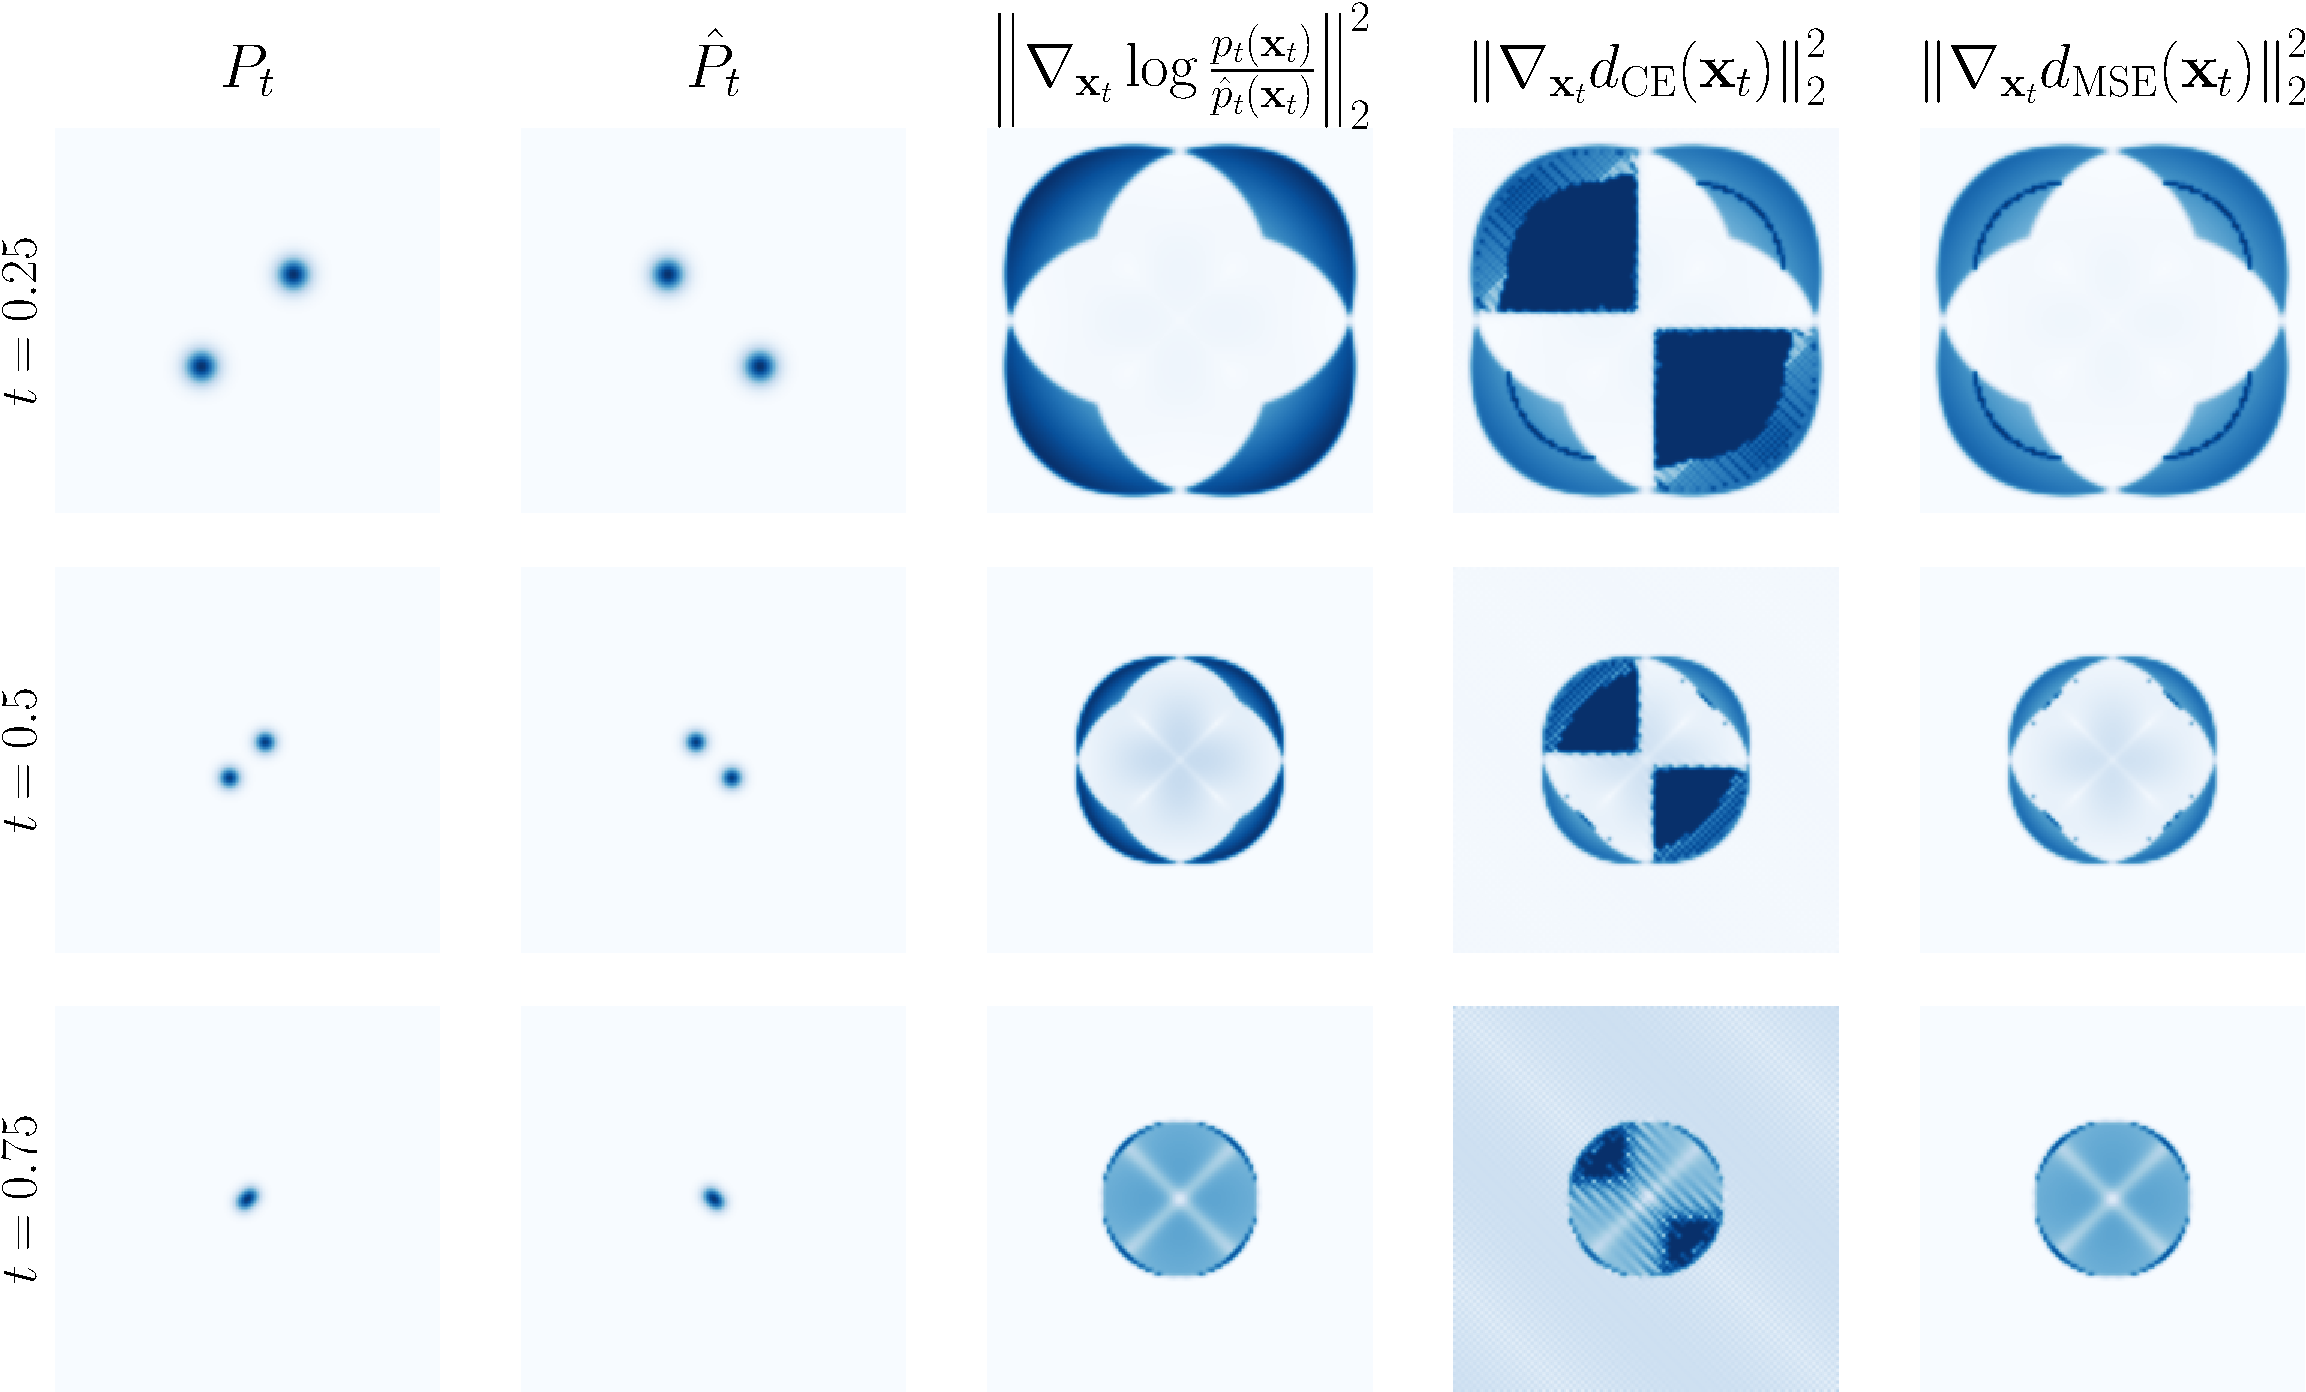
\includegraphics[width=\textwidth]{gfx/gradients_wrt_ts.pdf}
    \caption{Visualizing the estimation of $\nabla_{\vx_{t}} \log p_{t}(\vx_{t})/\nabla_{\vx_{t}} \log \hat{p}_{t}(\vx_{t})$ for the discriminator trained with low cross-entropy or low MSE loss. We plot the norm of the gradient for better readability. We can see here that the discriminator trained on minimizing $\mathcal{J}_{CE}$ provides a poor estimate of the gradient, while the one trained on $\mathcal{J}_{MSE}$ provides a sound estimate.}
    \label{fig:2d_gradient}
\end{figure}
\begin{figure}[t!]
    \centering
    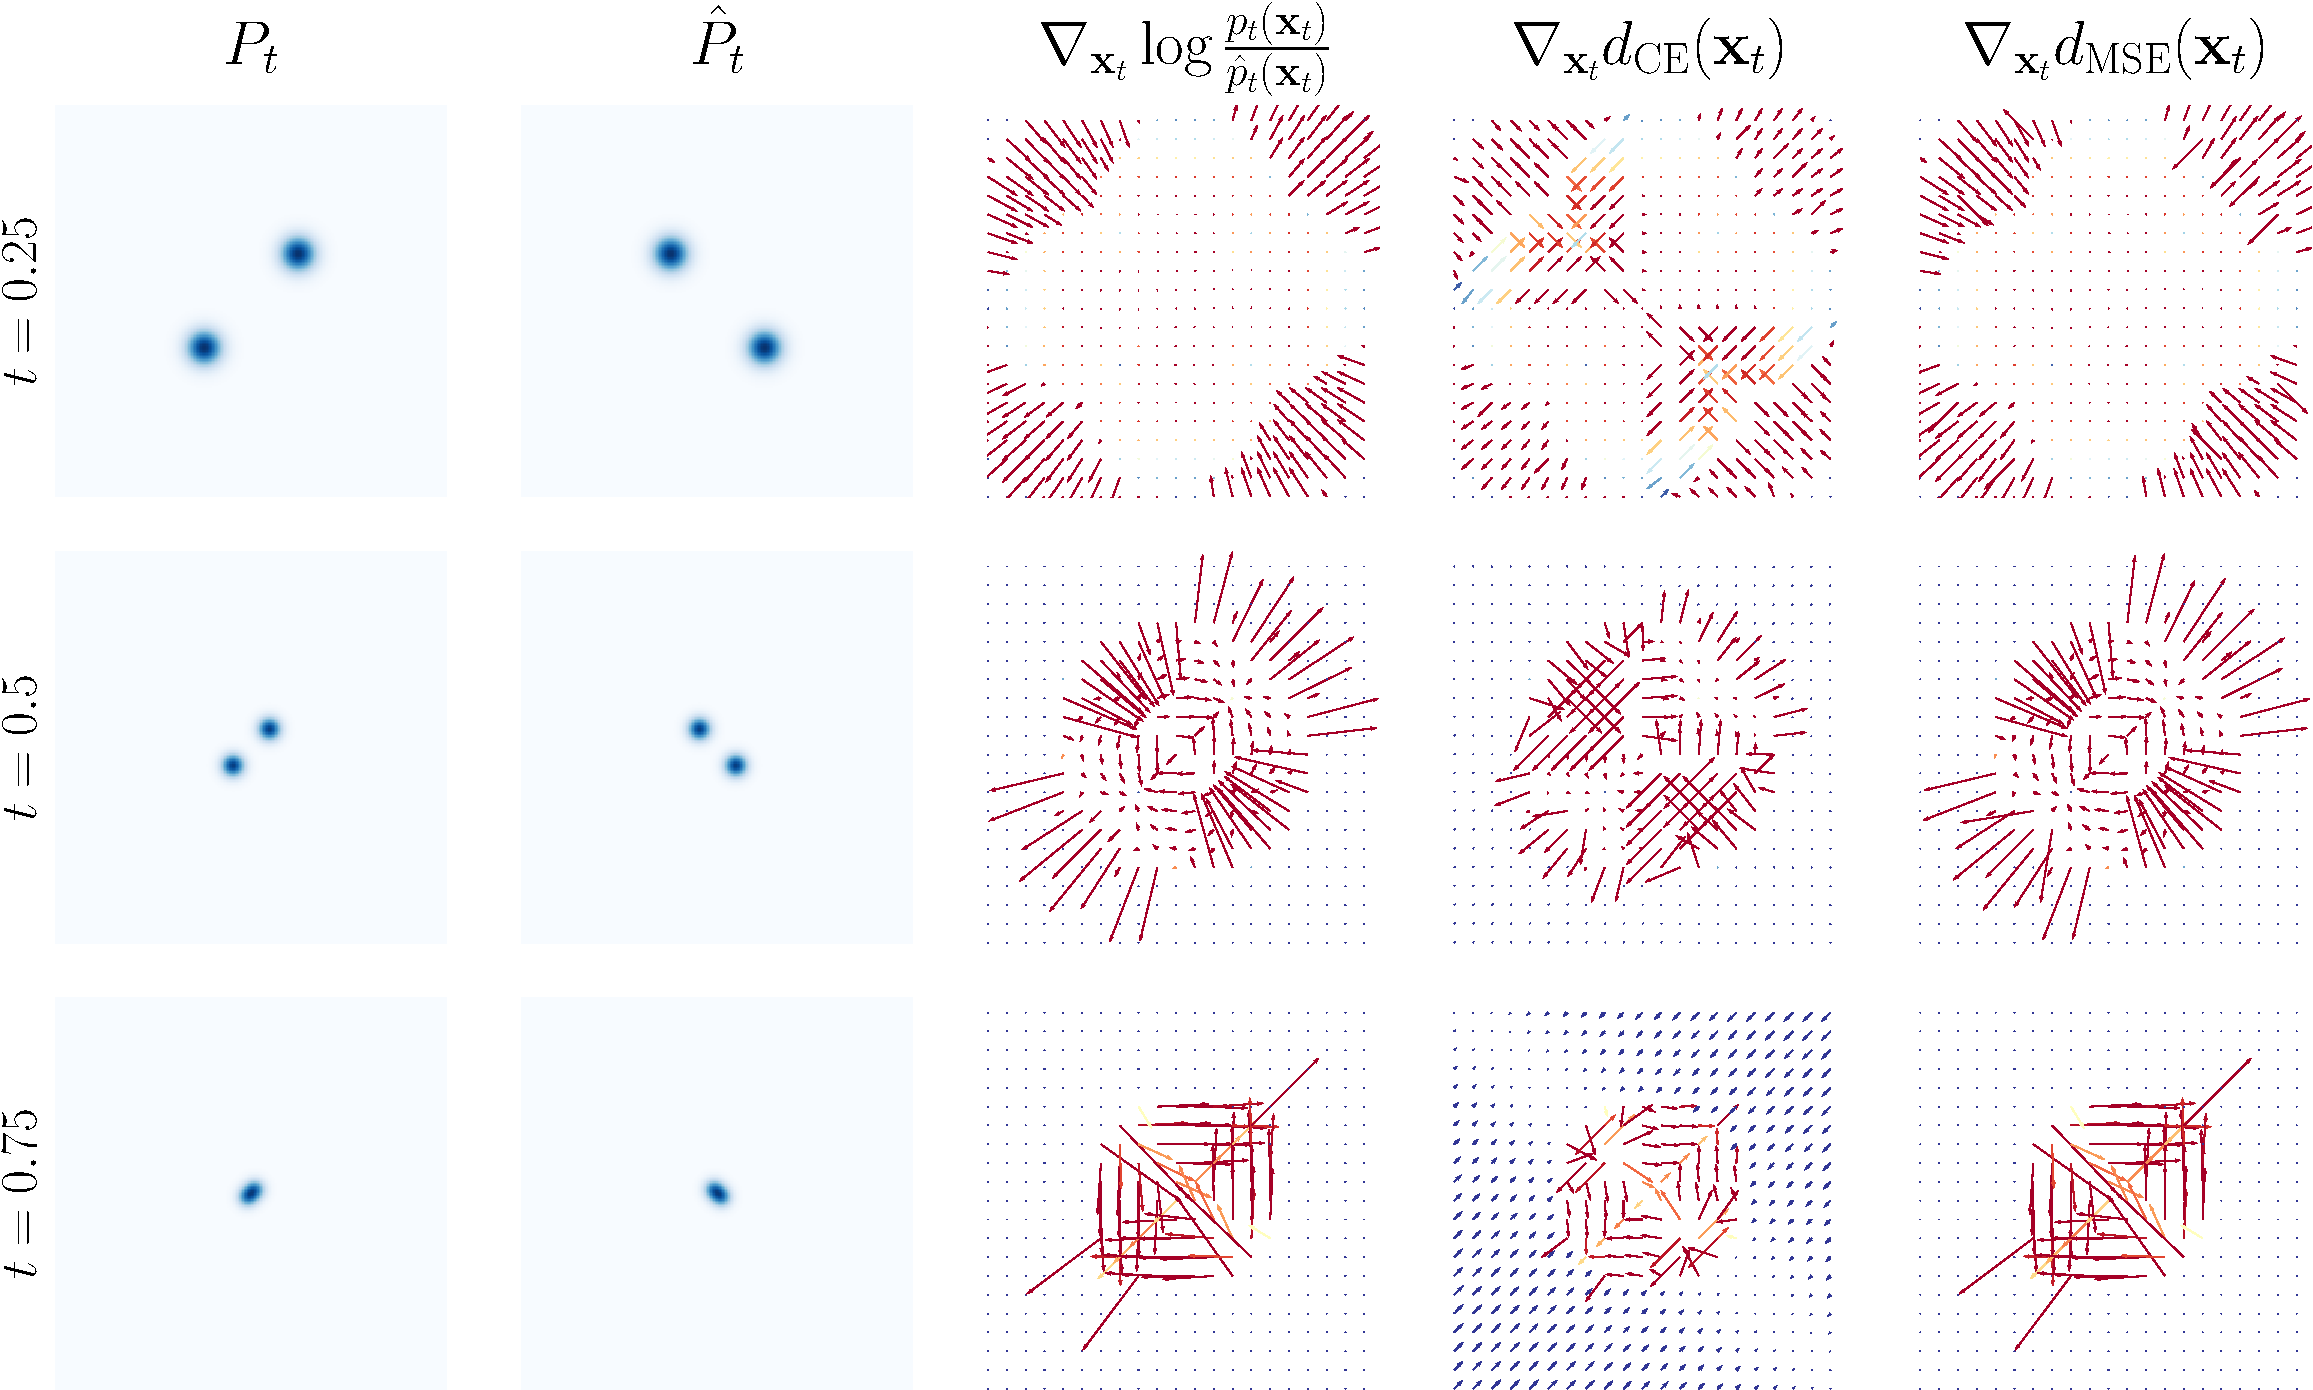
\includegraphics[width=\linewidth]{gfx/quivers_wrt_ts.pdf}
    \caption{Gradients of the estimated density ratio. $d_{\mathrm{CE}}$ represents a discriminator with low cross entropy, and $d_{\mathrm{MSE}}$ represents a discriminator with low MSE}
    \label{fig:2D-quivers}
\end{figure}
\subsection{Practical considerations}
One advantage proposed by the approach of \citep{kim2023refininggenerativeprocessdiscriminator} is the usage of generated samples from $\Hat{P}$ at each training step. 
Training a discriminator to minimize the MSE loss is more prone to overfitting, as no new samples are generated during training, as opposed to the cross-entropy loss. Furthermore, as our work focused on improving generation for already well trained model, the error $\nabla \log \frac{p_{t}(x)}{\tilde{p}_{t}(x)}$ is small. We thus propose to use leverage the generative abilities of the pretrained diffusion model $s_{\theta}$ to gain more information, by adding $\mathcal{J}_{CE}$ as a regularization term: 
\begin{equation}
    \mathcal{J}_{\mathrm{train}}(\phi) = \mathcal{J}_{\mathrm{MSE}}(\phi) + \gamma\mathcal{J}_{\mathrm{CE}}(\phi)
\end{equation}
where $\gamma$ is a hyperparameter controlling the regularization strength.
\section{Experiments}
\subsection{Toy example}

\textbf{Setting:}We consider two distinct mixtures of Gaussians in $\reals^{2}$, that represent respectively $P$ and $\tilde{P}$. We compute for a subset of timesteps $t \in [0,1]$ the closed form of the scores $\nabla_{\vx_{t}} \log p_{t}(\vx_{t})$ and $\nabla_{\vx_{t}} \log p_{t}(\vx_{t})$, and we use them for performing a discretized backward diffusion process. In order to concentrate on the effect of discriminator guidance, we first sample points from $P$, perform a forward diffusion process using subVP-SDE \citep{song2021scorebasedgenerativemodelingstochastic}, and start from this set of points as a prior distribution. 
\begin{figure}[b!]
    \centering
    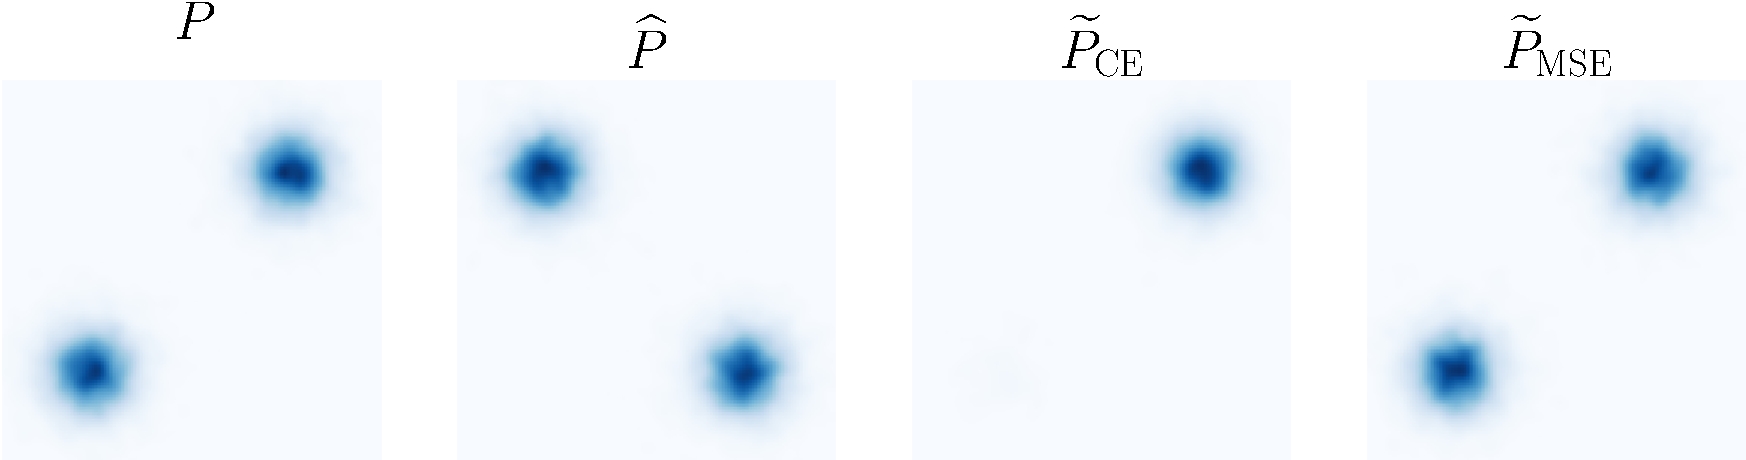
\includegraphics[width=\textwidth]{gfx/3_scenarios_omega_1e4.pdf}
    \caption{Comparison of the sampling process by using a discriminator to minimize the cross-entropy loss defining a distribution $\Tilde{P}_{\mathrm{CE}}$ and a discriminator to minimize the MSE loss $\mathcal{J}_{\mathrm{SM}}(\phi)$ defining a distribution $\Tilde{P}_{\mathrm{MSE}}$. We can see that the cross entropy loss misses one mode of the target distribution}
    \label{fig:2Dplots}
\end{figure}

\textbf{Evaluation of the optimization procedure :}
We also compute two estimations of the discriminator. The first estimate $d_{\mathrm{CE}}$ is based solely on minimizing $\mathcal{J}_{\mathrm{CE}}$ and the second $d_{\mathrm{MSE}}$ ensures a small $\mathcal{J}_{\mathrm{MSE}}$. We plot in Figure \ref{fig:2d_gradient} the gradient estimates across the denoising process and show that the discriminator estimated by minimizing the cross-entropy has a bad gradient estimate. Figure \ref{fig:2Dplots} shows that the failure to accurately estimate the gradient is detrimental to the denoising process. We also provide in Appendix \ref{fig:2D-quivers} the gradient plots of the different estimates.
\begin{figure}[b!]
    \centering
    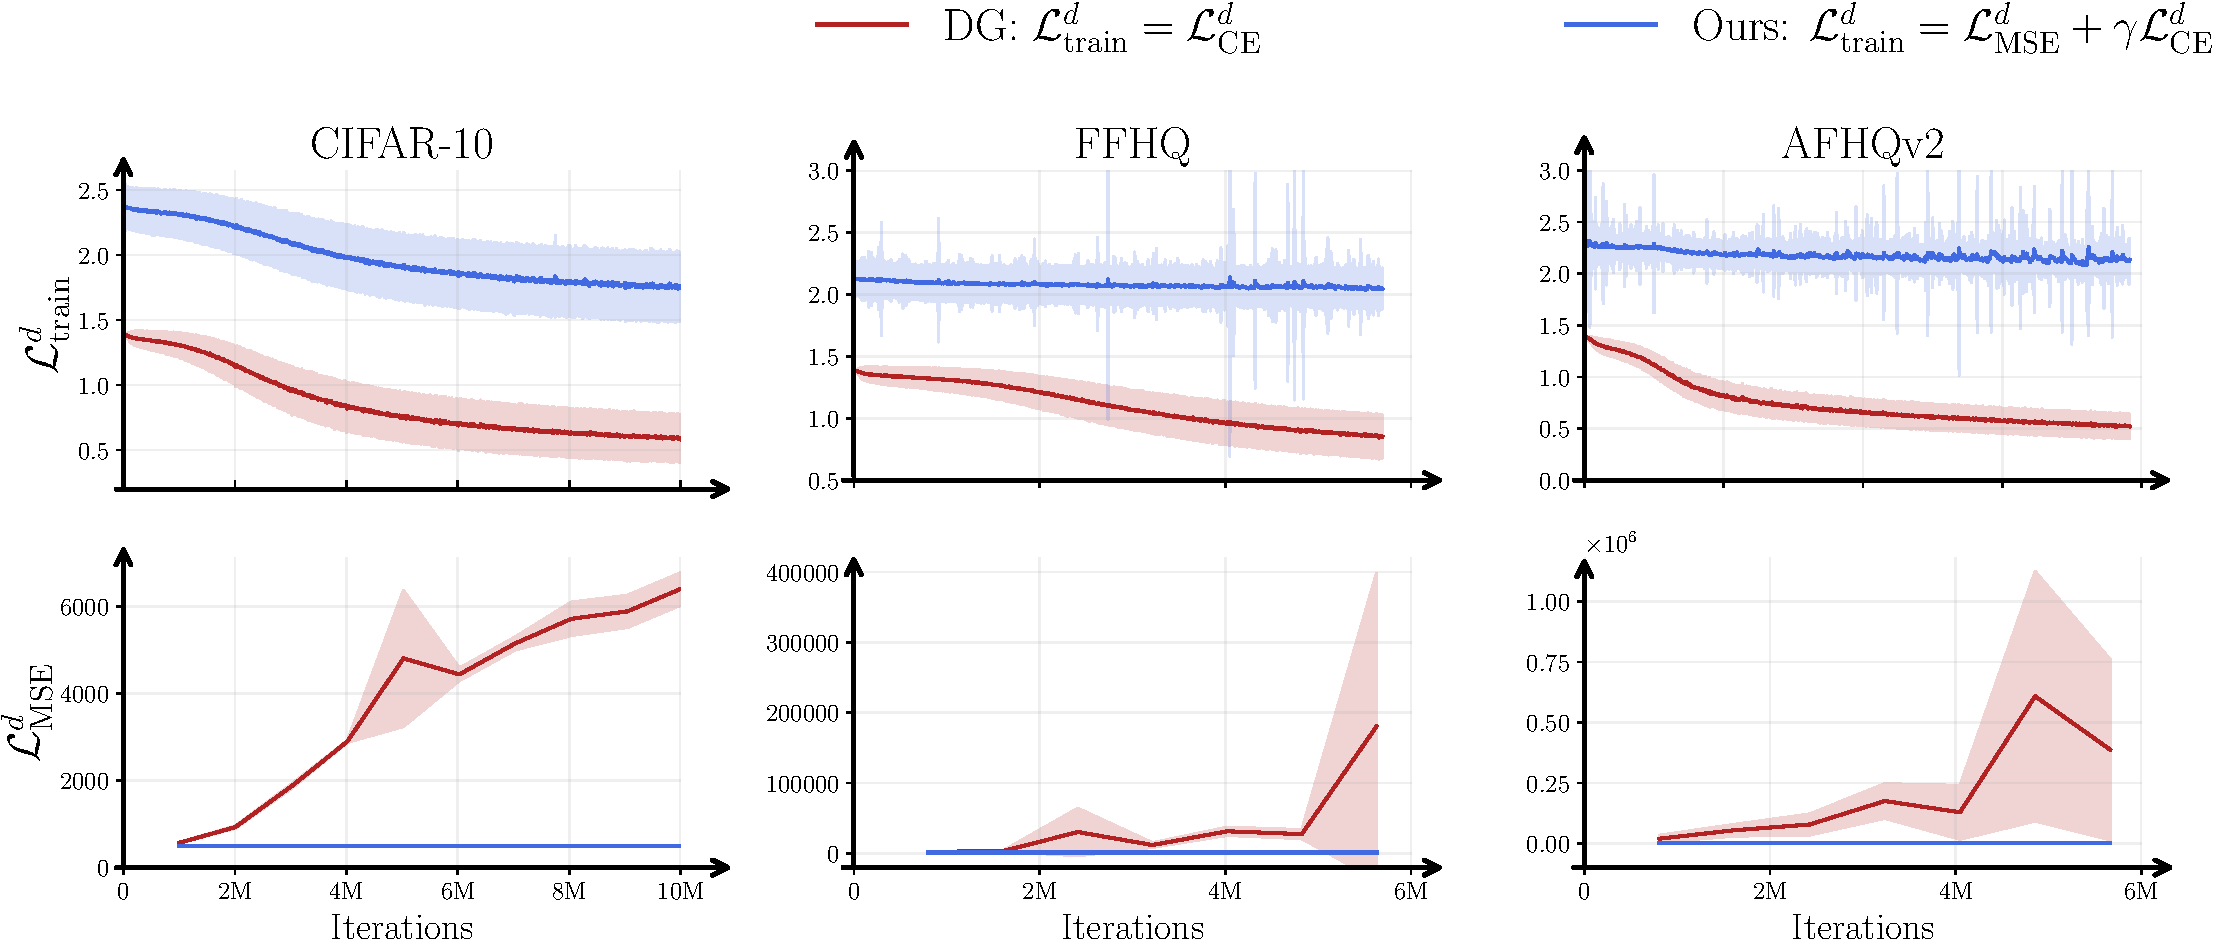
\includegraphics[width=\textwidth]{gfx/losses_DGvsOurs.pdf}
    \caption{Comparison of the proposed method with the method of \citet{kim2023refininggenerativeprocessdiscriminator} on the EDM model \citep{karras} on CIFAR-10, FFHQ and AFHQ-v2 datasets. For the method proposed by \citet{kim2023refininggenerativeprocessdiscriminator}, denoted as DG, the MSE loss $\mathcal{J}_{\mathrm{MSE}}$ increasing during training. The proposed method, denoted as Ours, shows a stable behavior. The error bars represent the standard deviation over 3 runs.}
    \label{fig:losses}
\end{figure}
\subsection{Image generation}
We implement our approach using the pre-trained EDM model \citep{karras}. We will compare our approach with the pre-trained models (EDM) and the pre-trained models with discriminator guidance (EDM+DG). For a fair comparison to \cite{kim2023refininggenerativeprocessdiscriminator}, we build the same architecture for the discriminator $d_\phi$ using pre-trained embedding of the ADM classifier models used in the work of \citet{dhariwal2021diffusionmodelsbeatgans}. However, our method requires using the same framework as EDM, therefore we reimplemented DG for various datasets and resolutions. We use the same hyperparameters as \citet{kim2023refininggenerativeprocessdiscriminator} for the discriminator guidance method, and we apply both methods on the CIFAR-10, FFHQ and AFHQ-v2 datasets on, respectively, 8x GPU-V100, 8x GPU-A100 and 8x GPU-A100. First, we illustrate the behavior of the training loss ($\mathcal{J}_{\mathrm{CE}}$ for DG and $\mathcal{J}_{\mathrm{train}}$ for Ours) and the reconstruction loss during training in Figure~\ref{fig:losses}. We can see that our approach enables us to mitigate the increase of the MSE loss, while the DG method shows a clear increase of the loss. However, we observe a decrease in the training loss that demonstrates that the density ratio is learned.

We report the FID\footnote{Note that we can observe some discrepancies between the results in \cite{kim2023refininggenerativeprocessdiscriminator} due to the reimplementation of the framework to closely match the generative process of EDM} \citep{heusel_gans_2017}, Precision and Recall \citep{kynkaanniemi_improved_2019} scores in Table~\ref{tab:results}. Metrics are computed using the Guided Diffusion library \citep{dhariwal2021diffusionmodelsbeatgans} using 50k samples for CIFAR-10 and FFHQ, and 15k samples for AFHQ-v2. We use $k=5$ to compute the Precision and the Recall. We can see that our method systematically outperforms the DG method on all datasets even if the difference with the EDM model is small.    

\begin{table}[t]
\centering
\caption{Comparison of the proposed method with the method of \citet{kim2023refininggenerativeprocessdiscriminator} on CIFAR-10, FFHQ and AFHQv2. We give metrics averaged on 3 trainings procedure with one standard deviation.} \label{tab:results} 
\begin{tabular*}{\textwidth}{lcl@{\extracolsep{\fill}}ccc}
\toprule
Dataset & Resolution & Method & FID & P & R \\
\midrule
\multirow{3}{*}{CIFAR-10} &\multirow{3}{*}{{$32\times32$}}&  EDM & $2.03$ & $99.12$ & $76.84$\\
 && EDM + DG & $3.03 \pm 0.05 $ & $99.06 \pm 0.10 $ & $72.56 \pm 0.14 $ \\
 && EDM + Ours & $2.00 \pm 0.01 $ & $99.18 \pm 0.04 $ & $76.70 \pm 0.12 $ \\
\midrule
\multirow{3}{*}{AFHQv2} &\multirow{3}{*}{{$64\times64$}}&  EDM & $2.62$ & $99.92$ & $84.66$\\
 && EDM + DG & $2.66 \pm 0.02 $ & $99.92 \pm 0.00 $ & $83.70 \pm 0.22 $ \\
 && EDM + Ours & $2.61 \pm 0.00 $ & $99.92 \pm 0.00 $ & $84.62 \pm 0.01 $ \\
\midrule
\multirow{3}{*}{FFHQ} &\multirow{3}{*}{{$64\times64$}}&  EDM & $2.54$ & $99.75$ & $78.85$\\
 && EDM + DG & $2.63 \pm 0.03 $ & $99.74 \pm 0.02 $ & $77.55 \pm 0.06 $ \\
 && EDM + Ours & $2.54 \pm 0.00 $ & $99.75 \pm 0.00 $ & $78.87 \pm 0.02 $\\
\bottomrule
\end{tabular*}
\end{table}
\subsection{Comments on the results}
Training a discriminator to refine the EDM model \citep{karras} slightly improved the generation metrics, but the difference is not significant. We hypothesize that this is due to the fact that the EDM model is already well trained, and the discriminator guidance method is not able to provide a good estimate of the gradient of the log-density ratio. A more notable contribution would be to try this method on less trained models, and evaluate the improvement in FID, precision and recall. 
Thus, as future directions of this part, we propose the following : 
\begin{itemize}
    \item Our work also lacks the diversification of architectures, and should have been tried with other pre-trained models, for tasks different than image generation.
    \item Fine-tune the hyperparameter $\gamma$, or investigate other regularization terms to improve the training process.
    \item Restrict discriminator guidance to timesteps $t$ where the score estimation is poor.
    \item Investigate the effect of discriminator guidance on less trained models.
\end{itemize}

\section{Conclusion}\label{sec:dg:conclusion}
In this chapter, we presented a method for refining pre-trained diffusion models using a smaller discriminator network. After introducing the method proposed by \citep{kim2023refininggenerativeprocessdiscriminator}, we provided theoretical results that lead to modifying the training objective of the discriminator, and prove that our proposed objective is optimal.
We then provided experimental results to evaluate the validity of our approach, and showed that it was not effective for the EDM model. We provided future directions to improve the method. 
Discriminator guidance attempts to correct the \textit{approximation} errors related to the score estimation while training. Now, the following chapter answers the following question : \textbf{Can the sampling erros, related to the discretization of the backward process, be corrected by a boosting method ?}

	% INCLUDE: system
% !TEX root = ../thesis-example.tex
%
\chapter{Reinforcement Learning based methods}\label{sec:rl}
The idea of refining the sampling process of a diffusion model consists in correcting the sampling error related to the discretization of the backward SDE \ref{eq:backward_diffusion} or ODE. 
In section \ref*{sec:related:improve_generation}, we introduced \textit{rejection} sampling as a method to correct the sampling error. This method relies on using a trained discriminator to reject samples that are not close to the true distribution.
However, in high dimensions, the optimal acceptance probability of a sample becomes very small, which makes the rejection sampling method inefficient. We also would like to propose a method that is tailored for diffusion models, using the fact that the score network approximates the target distribution in different noise levels $t \in [0, T]$.
In the first section, we introduce restart sampling \citep{xu_restart_2023} as a \textit{boosting free} method to correct the sampling process. The method overall consists in improving the sampling process by solving the backward ODE \ref{eq:backward_diffusion}, renoising, and restarting the process for $K$ times. $K$ in this case is a hyperparameter that is manually tuned, thus raising the question of finding an optimal $K$ for a pre-trained diffusion model.
We propose to use Reinforcement Learning (RL) to instead dynamically noise / denoise the samples. We thus present briefly reinforcement learning in the second section, and formalize the problem for diffusion models in the third section. Experiments are currently ongoing for the end of the internship.




\section{Restart sampling}\label{sec:rl:sec1}
\subsection{Trade-off between speed and quality}
In order to sample from a diffusion model, the standard approach is to solve the backward ODE (Equation \ref{eq:backwatd_ode}) / SDE (Equation \ref{eq:backward_diffusion}) using numerical solvers, such as Heun's 2nd method and Euler-Maruyama's method \citep{kpj1992numerical}. The choice between reversing the ODE and the SDE is a trade-off between speed and quality : 
\begin{itemize}
    \item Sampling speed is evaluated for diffusion number by the number of function evaluations (NFE). That is, the number of calls to the score model $s_{\theta}$ during the sampling process. (Fast means low NFEs)
    \item Quality is commonly assessed by metrics depending on the data type. For image generation, the Fréchet Inception Distance (FID) \citep{heusel2017gans} is a common metric. (High quality means low FID)
\end{itemize}
As the sampling speed increases (low NFE), the sample quality generally deteriorates (high FID). This is explained by the discretization error caused by using a larger step size in numerical differential equation solvers.
As illustrated in figure \ref{fig:restart_sampling_nfe_quality}, ODE solvers are efficient in the small NFE regime, providing a decent quality with a large step size. They are outperformed by SDE solvers for smaller step sizes (high NFE) in terms of quality, and fail to improve when increasing the NFE.
\begin{figure}[htbp]
    \centering
    \begin{subfigure}{0.45\textwidth}
        \centering
        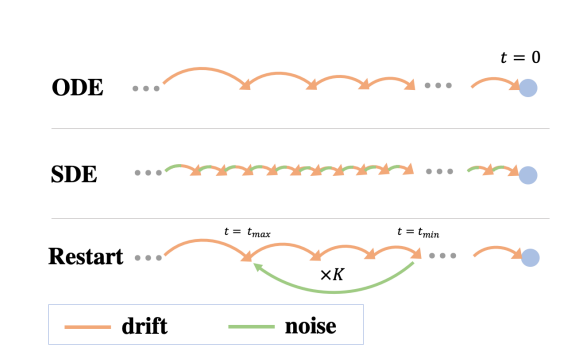
\includegraphics[width=\linewidth]{gfx/restart_sampling.png} % Left image
        \caption{Restart sampling method}
        \label{fig:restart_sampling}
    \end{subfigure}\hfill
    \begin{subfigure}{0.45\textwidth}
        \centering
        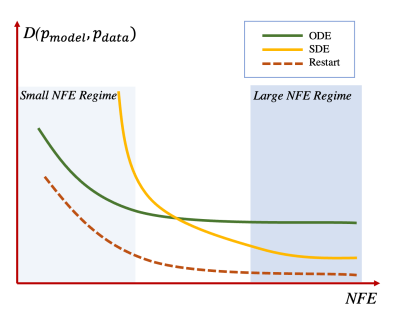
\includegraphics[width=\linewidth]{gfx/nfe_quality.png} % Right image
        \caption{Number of function evaluations (NFE) vs sampling quality}
        \label{fig:nfe_quality}
    \end{subfigure}
    \caption{Taken from \citep{xu_restart_2023}. \textbf{\ref*{fig:restart_sampling}} Illustration of restart sampling. \textbf{\ref*{fig:nfe_quality}} Sample quality vs NFE for different numerical solvers. ODE solvers (green) allow for a better quality than SDE solvers (yellow) in the small NFE regime, but plateau quickly in the large NFE regime.}
    \label{fig:restart_sampling_nfe_quality}
\end{figure}
\subsection{Sampling with ODE solvers vs SDE solvers}
In the small NFE regime, the effectiveness of ODEs can be explained by comparing the local error of the two methods. For a step size $\delta$, the Euler method for solving ODEs yields a local error of $O(\delta)^{2}$, while the Euler-Maruyama method for solving SDEs yields a local error of $O(\delta^{\frac{3}{2}})$ \citep{Dalalyan_2019}. 
In the large NFE regime, the step size $\delta$ becomes small thus the discrepancy between the two local errors becomes negligible. The main source of error thus becomes the \textit{approximation} error of the score model $s_{\theta}$. Intuitively, adding noise by solving the SDE corrects the approximation error. The absence of a noise term in the ODE solvers thus can be explained by the domination of the approximation error over the discretization error, that cannot be corrected via noise.
\citep{xu_restart_2023} provide a theorem that formalizes the behaviour difference between the two methods : 
\begin{theorem}\citep{xu_restart_2023}
Let $[t_{\min},t_{\max}] \subset [0,T] $, and let $\tilde{p}_{t}^{ODE}, \tilde{p}_{t}^{SDE}$ denote the distributions of simulating the ODE and SDE respectively, with the estimated score $s_{\theta}$. Assume for a given $B$
that $\forall t \in [t_{\min},t_{\max}], \|x_{t}\| \leq \frac{B}{2}$ for any $x_{t}$ in the support of $P_{t},\Tilde{P}_{t}^{ODE},\Tilde{P}_{t}^{SDE}$. Then we have the following upper bounds :
\begin{align}

    W_{1}(\tilde{p}_{t_{\min}}^{ODE},p_{t_{\min}}) &\leq B \cdot TV(\tilde{p}_{t_{\max}}^{ODE},p_{t_{\max}}) + O(\delta + \varepsilon_{\mathrm{approx}})(t_{\max}-t_{\min}) \\
    W_{1}(\tilde{p}_{t_{\min}}^{SDE},p_{t_{\min}}) &\leq \underbrace{(1-\lambda e^{-U})}_{\mathrm{contraction term}}\cdot B \cdot TV(\tilde{p}_{t_{\max}}^{SDE},p_{t_{\max}}) + O(\sqrt{\delta t_{\max}} + \varepsilon_{\mathrm{approx}})(t_{\max}-t_{\min})

\end{align}
where $W_{1}(.,.)$ denotes the 1-Wasserstein distance, $TV(.,.)$ denotes the total variation distance, $U = \frac{BL_{1}}{t_{\min}} + \frac{L_{1}^{2}t_{\max}^{2}}{t_{\min}^{2}}$, $\lambda < 1$ is a contraction factor, $L_{1}$ and $\varepsilon_{\mathrm{approx}}$ are uniform bounds on $\|ts_{\theta}(x,t)\|$ and the approximation error $\|ts_{\theta}(x,t) - t\nabla_{x} \log p_{t}(x)\|$ respectively.
\end{theorem}
Both right hand sides of the inequality feature two distinct terms in a sum. The first term denotes the \textit{contracted} error, i.e the initial errors
accumulated from both approximation and discretization errors during the simulation of the backward
process, up until time $t_{\max}$. The second term denotes the \textit{additional sampling} error. This term is essentially the same for both inequalities as $\delta$ gets small, but the contraction error is lowered by the term $U$ as the denoising process progresses, explaining the role of the noise in correcting the approximation error. 
This raises the following question : 
\textbf{Is there a sampling procedure that maintains the same discretization error as ODE solvers, while correcting the approximation error as SDE solvers do ?}

\subsection{Solving back and forth}
\citep{xu_2023_restart} propose \textit{restart sampling}, a sampling technique consisting in doing back and forth steps during the sampling process during a pre-defined time interval $[t_{\min},t_{\max}] \subset [0,T]$. As depicted in figure \ref{fig:restart_sampling}, a restart backward step consists in performing an ODE step from $t$ to $t-1$. A restart forward step consists in adding noise following the diffusion forward process (Equation \ref{eq:forward_diff}) from time $t_{\min}$ to time $t_{\max}$. This process is repeated $K$ times, and the final sample is the output of the last ODE backward step, from $t_{\min}$ to 0.
The authors provide the following upper bound on the 1-Wasserstein distance between the \textit{refined} distribution $Tilde{P}_{t_{\min}}^{\mathrm{restart}}$ and the target distribution $P_{t_{\min}}$:
\begin{equation}
    W_{1}(\Tilde{P}_{t_{\min}}^{\mathrm{restart}},P_{t_{\min}}) \leq B \cdot (1 - \lambda)^{K}TV(\Tilde{P}_{t_{\max}}^{\mathrm{restart}},P_{t_{\max}}) + (K+1) O(\delta + \varepsilon_{\mathrm{approx}})(t_{\max}-t_{\min})
\end{equation}
This inequality combines both advantages of ODE solvers (lower second term) and SDE solvers (approximation error contraction, exponential in $K$). 
However, this method introduces two additional degrees of freedom : the choice of the value of $K$ and the restart interval $[t_{\min},t_{\max}]$. This raises the following question : 
\textbf{Is it possible to dynamically noise / denoise the samples, without the need to manually tune $K$ ?}
We explore the option of using reinforcement learning as method to dynamically noise / denoise the samples, and present the formalization of the problem in the next section.
\section{Reinforcement Learning }\label{sec:rl:sec2}
\subsection{Background}
Reinforcement learning is a machine learning paradigm that stems from control theory. It essentially attempts to learn an optimal \textit{policy}, which is a probability distribution over actions given an observed state.
It is described by a markov decision process (MDP) tuple $(S, A, T, R, \gamma )$, where :
\begin{itemize}
    \item S is the set of states of the environment, that can either be continuous or discrete
    \item A is the set of actions that the agent can take
    \item T is the transition model such that $T(s'| s,a ) = P(S_{t+1} = s' | S_t = s , A_t = a)$
    \item R is the reward function that gives the reward r after taking action $a$ in state $s$
    \item $\gamma$ is the discount factor
\end{itemize}
A reinforcement learning \textit{agent} interacts with the environment during episodes. Given $s_{0} \sim \mu_{0}$, where $\mu_{0}$ is the distribution over initial states, the agent takes an action $a_{0}$ according to its policy $\pi_{\psi}$, and receives a reward $r_{0}$ and a new state $s_{1}$. The process is repeated until a terminal state is reached. The goal of the agent is to learn the optimal policy $\pi^{*}$ that maximizes the expected return :
\begin{equation}
    \mathcal{J}_{\mathrm{RL}}(\psi) = \mathbb{E}_{\pi_{\psi}}[\sum_{t=0}^{\infty} \gamma^{t}r_{t}]
\end{equation}
We denote by $\tau = (s_{0},a_{0},r_{0},s_{1},a_{1},r_{1},\ldots,s_{L})$ the trajectory of the agent by running an episode simulation in the environment.
The field of RL has gained a lot of attention in the past decade, with the advent of deep reinforcement learning involving deep neural networks \citep{mnih2013playingatarideepreinforcement}. It has been applied to several tasks, notably robotics \citep{gupta2019relaypolicylearningsolving}, protein synthesis \citep{jumper2021highly}, and famously for allowing the safe and aligned deployment of large language models through Reinforcement Learning from Human Feedback (RLHF) \citep{ouyang2022traininglanguagemodelsfollow}.
Several methods were developed to solve reinforcement learning, such as Q-learning, policy gradient methods, and actor-critic methods. Our work focuses on policy-gradient methods, and more specifically on the Proximal Policy Optimization (PPO) algorithm \citep{schulman2017proximal}. We present in the following section a modified version of the PPO algorithm that relies on $f-$divergences.
\subsection{Matching state visitation distributions}
The distribution over trajectories induced by the policy $\pi_{\psi}$ can be defined by the density : 
\begin{equation}
    p_{\psi}(\tau) = \mu_{0}(s_{0})\prod_{t=0}^{L-1} \pi_{\psi}(a_{t}|s_{t})p(s_{t+1}|s_{t},a_{t})
\end{equation}
Thus, the distribution over states induced by the policy $\pi_{\psi}$ can be defined by the density :
\begin{align}
    p_{\psi}(s) &= \frac{\int p_{\psi}(\tau)\eta_{\tau}(s) d\tau}{Z} \\
    &= \frac{\int \mu_{0}(s_{0})\prod_{t=0}^{L-1} \pi_{\psi}(a_{t}|s_{t})p(s_{t+1}|s_{t},a_{t})\eta_{\tau}(s)}{\int \int \mu_{0}(s_{0})\prod_{t=0}^{L-1} \pi_{\psi}(a_{t}|s_{t})p(s_{t+1}|s_{t},a_{t})\eta_{\tau}(s) d\tau ds } d\tau
\end{align}
with $\eta_{\tau}(s) = \sum_{s_{t} \in \tau } \delta(s - s_{t})$ the number of occurences of state $s$ in trajectory $\tau$.
As a result, the optimal policy similarly defines a disribution over state visitation, that we write as $P^{*}$ with density $p^{*}(s)$. This allows to formulate the following objective function :
\begin{equation}\label{eq:rl:learning_problem}
    \mathcal{J}_{\mathrm{RL}}(\psi) = D_{f}(p_{\theta},p^{*})
\end{equation}
\subsection{f-Policy gradient}
As explained in section \ref*{sec:rl:sec3}, this formulation allows to find an optimal policy without access to the reward function. This is crucial in our case since in the context of refining diffusion models, the only information we have are samples from the target distribution $P_{t}$ and the estimated score $s_{\theta}$.
Computing the $f-$divergence in equation \ref{eq:rl:learning_problem} is intractable, but \citep{agarwal_f-policy_2023} derive an expression for its gradient, in a similar flavor to the policy gradient theorem \citep{NIPS1999_464d828b} :
\begin{equation}
    \nabla  \mathcal{J}_{\mathrm{RL}}(\psi) =  \mathbb{E}_{P_{\psi}} \left[ \left( \sum_{t=1}^{L} \nabla_{\psi} \log \pi_{\psi}(a_{t}|s_{t})  \right) \left(\sum_{t=1}^{L}f'\left( \frac{p_{\psi}(s_{t})}{p_{*}(s_{t})} \right)   \right)   \right]
\end{equation}

In practice, computing this gradient is computationally intensive since it requires performing \textit{on policy} updates. That is, the policy used to interact with the environment is updated on the go. This is not feasible for complex environments, as learning quickly becomes sample inefficient.
In order to enforce off-policy learning, one idea \citep{agarwal_f-policy_2023} was to use importance sampling from another policy $\pi_{\psi'}$ to estimate the gradient. In order to provide a good estimation, the current policy $\pi_{\psi}$ and the estimating policy $\pi_{\psi'}$ should be close. This is enforced by the Proximal Policy Optimization (PPO) algorithm \citep{schulman2017proximal}, that constrains the policy update to a certain distance from the previous policy. This is done by clipping the ratio of the new policy to the old policy, and using the clipped ratio to compute the loss function. This leads to the following expression for the gradient of $\mathcal{J}_{\mathrm{RL}}(\psi)$ :
\begin{equation}
    \nabla  \mathcal{J}_{\mathrm{RL}}(\psi) =  \mathbb{E}_{(s_{t},a_{t}) \sim P_{ \psi'}} \left[  \min\left(r_{\psi}(s_{t},a_{t})F_{\psi'}(s_{t}),\mathrm{clip}\left(r_{\psi}(s_{t},a_{t}),1-\varepsilon,1+\varepsilon\right)F_{\psi'}(s_{t}) \right)  \right]
\end{equation}
where $r_{\psi}(s_{t},a_{t}) = \frac{\nabla_{\psi} \pi_{\psi}(a_{t}|s_{t})}{\pi_{\psi'}(a_{t}|s_{t})}$ is the importance sampling ratio, $F_{\psi'}(s_{t}) = \sum_{i=t}^{T} \gamma^{i} f'\left( \frac{p_{\psi'}(s_{i})}{p_{*}(s_{i})} \right)$, and $\varepsilon$ is a hyperparameter that controls the clipping of the ratio. Algorithm \ref*{alg:fpg} describes the generic training procedure for a given environment, and samples from the expert policy.
\begin{algorithm}
    \caption{f-PG}
    \label{alg:fpg}
    \begin{algorithmic}[1]
    \State Let $\pi_\psi$ be the policy, $B$ be a buffer, $\mathcal{S}$ the set of trajectories from the expert policy
    \For{$i = 1$ to $\text{num\_iter}$}
        \State $B \leftarrow []$
        \For{$j = 1$ to $\text{num\_traj\_per\_iter}$}
            \State Simulate trajectory $\tau$ using $\pi_\psi'$
            \State Train a discriminator $d_{\phi}$ to estimate the density ratio $\frac{p_{\psi'}(s)}{p_{*}(s)}$
            \State Store $f' \left( d_{\phi}(s) \right)$ for each $s$ in $\tau$
            \State $B \leftarrow B + \{\tau \}$
        \EndFor
        \For{$j = 1$ to $\text{num\_policy\_updates}$}
            \State $\theta \leftarrow \theta - \alpha \nabla_\psi J_{\mathrm{RL}}(\psi)$
        \EndFor
    \EndFor
    \end{algorithmic}
    \end{algorithm}
In the following section, we will devise a procedure to apply the f-PG algorithm to the problem of refining diffusion models.

\section{Application to diffusion models}\label{sec:rl:sec3}
\subsection{Formalizing the restart sampling problem as a reinforcement learning problem}
The sampling process of diffusion models can be seen as a trajectory in the state space of a reinforcement learning agent. We train an agent to decide whether an ODE denoising step can be done, or if noise should be added to the current sample. The goal of the agent is to minimize the $f-$divergence between the state visitation distribution of the current policy and the optimal policy: 
\begin{itemize}
    \item  The state space can be defined as the set of samples $x_{t}$ of the discretized denoising process. Note that the timestep $t$ refers to the noise level in the diffusion model. To make a difference with the time variable in the reinforcement learning context, we will refer to the RL timestep as $l$.
    \item The action space is discretized in two actions : perform one ODE denoising step to go from $x_{t}$ to $x_{t-1}$, or perform add noise to go from $x_{t}$ to $x_{t+1}$.
    \item The trajectory length is a fixed number of steps $L \geq T$
    \item The reward function is the $f-$divergence between the state visitation distribution of the current policy and the optimal policy.
    \item The samples from the expert (optimal) policy are the samples from the target distribution $P_{t}$. Each sample $x_{t}$ is obtained from samples $x_{0}$ from the initial distribution $P_{0}$ (dataset), diffused according to the forward diffusion equation (Equation \ref{eq:forward_diff}) up to time $t$.
\end{itemize}
Up to the current stage of the thesis, this approach is exploratory and we lacked time to provide theoretical guarantees on the validity of this method. The following section describes the training procedure, that we term as \textit{f-Restart sampling}.
\subsection{f-Restart sampling}
We train a neural network that represents the policy $\pi_{\psi}$ to output a probability distribution over the set of actions \{Noise,ODE step\}. We train the policy using the f-PG algorithm, with the discriminator $d_{\phi}$ estimating the density ratio $\frac{p_{\psi'}(s)}{p_{*}(s)}$. The training dataset $\mathcal{S}$ is composed of samples from the target distribution $P_{t}$, and the buffer $B$ is used to store the trajectories of the agent. The training process is done for a fixed number of iterations, with a fixed number of trajectories per iteration, and a fixed number of policy updates per iteration. The hyperparameters $\alpha$ and $\varepsilon$ are manually tuned. The training process is done in an off-policy manner, with the policy $\pi_{\psi'}$ used to generate the trajectories. The training procedure is summarized in Algorithm \ref{alg:frs}

\begin{algorithm}
    \caption{f-Restart sampling}
    \label{alg:frs}
    \begin{algorithmic}[1]
    \State Let $\pi_\psi$ be the policy, $B$ be a buffer, $\mathcal{S}$ denote the training dataset (samples from the target distribution)
    \For{$i = 1$ to $\text{num\_iter}$}
        \State $B \leftarrow []$
        \For{$j = 1$ to $\text{num\_traj\_per\_iter}$}
            \State sample $x_{T}^{0}$ from the prior distribution $\mathcal{N}(0,I_{d})$
            \State $x_{0} \leftarrow x_{T}^{0}$
            \State $t_{0} \leftarrow T$
            \For{$l = 1$ to $L$}
            \State Compute $\pi_{\psi}(a|x_{l})$ for each action $a \in \{ \text{Noise, ODE step} \}$ and choose the action with highest probability
            \If {action = Noise}
                \State $x_{l+1} \leftarrow  $ Noise $x_{t}^{l}$ following the forward diffusion process
                $t_{l+1} \leftarrow t_{l} + 1$
            \Else
                \State $x_{l+1} \leftarrow  $ Perform one step of ODE denoising
                $t_{l+1} \leftarrow t_{l} - 1$
            \EndIf
            \State Store $(x_{l},t_{l},a_{l},x_{l+1},t_{l+1})$ in $\tau$
            \EndFor
            \State Train a discriminator $d_{\phi}$ to estimate the density ratio $\frac{p_{\psi'}(s)}{p_{*}(s)}$
            \State Store $f' \left( d_{\phi}(s) \right)$ for each $s$ in $\tau$
            \State $B \leftarrow B + \{\tau \}$
        \EndFor
        \For{$j = 1$ to $\text{num\_policy\_updates}$}
            \State $\theta \leftarrow \theta - \alpha \nabla_\psi J_{\mathrm{RL}}(\psi)$
        \EndFor
    \EndFor
    \end{algorithmic}
    \end{algorithm}
During this procedure, the quantities $f' \left( d_{\phi}(s) \right)$ can be seen as a guiding signal for the sampling algorithm to correct the approximation error. If at a denoising timestep $t$ this signal is low, then the agent should add noise to the sample to correct the error, thus using the advantage of SDEs introduced in section \ref*{sec:rl:sec1}. A high signal encourages the agent to continue the ODE denoising process.

\subsection{Experiments and results}
In order to test our proposed method, we will use a toy example of a 2D DDPM diffusion model. The target distribution is a mixture of 10 isotropic Gaussians, and we consider a trained score network that is trained on a samples stemming from a subset of modes of the target distribution. We use $f(u) = u\logu$ for minimizing the KL divergence between the target distribution and the state visitation distribution.
The first problematic behaviour observed is that the policy $\pi_{\psi}$ favours the noising step over the ODE denoising step. After one training epoch, the probability of choosing the noise action is close to 1. This was expected as the distributions $P_{t}$ and $\Tilde{P}_{t}$ are very close when the noise step is high. A workaround to this issue is to use a \textit{shaping} technique, consisting in encouraging the agent in the initial stages of training to perform the ODE denoising step.
\\
\textbf{Time weighting :} In order to force the agent to perform the ODE denoising step at the inital stages of training, we add a denoising time weighting factor to the density ratio, which essentially puts more importance to the smaller values of $t$. In our experiments, we choose a weighting term $w(t)$ that is linearly decreasing with $t$.
The effect of this shaping method was quite strong, and induced the reverse problematic behaviour : the agent would perform the ODE denoising step at each timestep. A few tweakings on the weighting scheme $w(t)$ were attempted, but the results were not satisfactory.
Figure \ref{fig:shaping_effect} shows that the agent does not change its behaviour post training, resulting in not improving the sampling process. We conclude that our shaping method was not effective, and provide the following directions for future work :
\begin{figure}[htbp]
    \centering
    \begin{subfigure}{0.32\textwidth}
        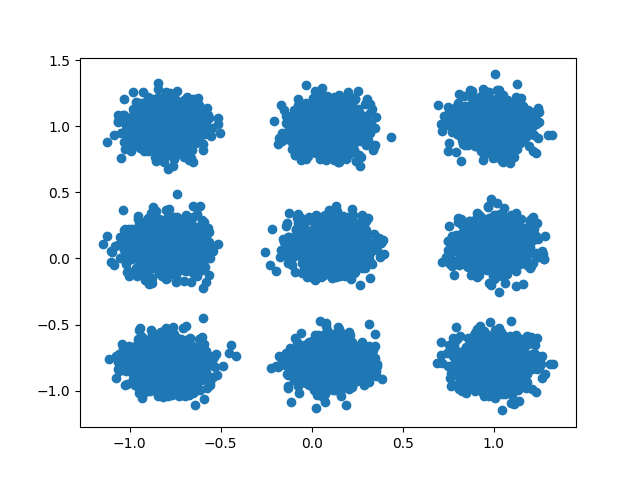
\includegraphics[width=\linewidth]{gfx/Real Data.png}
        \caption{Target distribution}
        \label{fig:target_samples}
    \end{subfigure}
    \hfill 
    \begin{subfigure}{0.32\textwidth}
        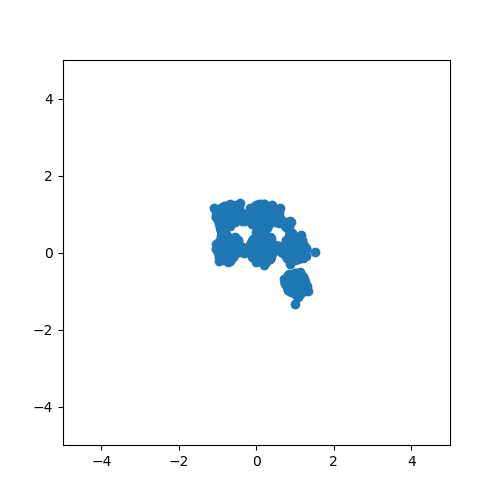
\includegraphics[width=\linewidth]{gfx/rl_before_train.png}
        \caption{Samples from $\Tilde{P}$ before training}
        \label{fig:pre_trained}
    \end{subfigure}
    \hfill 
    \begin{subfigure}{0.32\textwidth}
        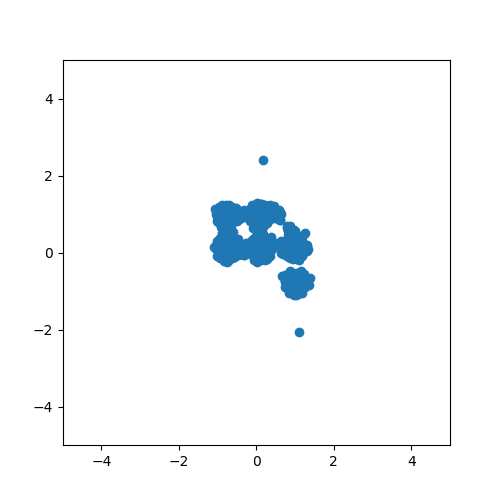
\includegraphics[width=\linewidth]{gfx/exponential_False_plots_rl_train_50.png}
        \caption{Samples from $\Tilde{P}$ after training}
        \label{fig:shaping}
    \end{subfigure}

    \caption{Reward shaping effect on the samples}
    \label{fig:shaping_effect}
\end{figure}
\begin{itemize}
    \item The optimality of the f-Restart sampling procedure was not proven. Further exploration on the theoretical aspect are needed to provide better insights for designing a training algorithm.
    \item Other shaping techniques should be considered to encourage the agent to perform the ODE denoising steps for high noise levels, but less frequently for low noise levels.
    \item Reinforcement learning relies on the Markov stationarity assumption, which might not be satisfied by our formulation of the state space. A more careful design of the state space should be considered.
\end{itemize}
\section{Conclusion}\label{sec:rl:conclusion}
In this chapter, we introduced the restart sampling method as a way to correct the sampling error of diffusion models. We then proposed to use reinforcement learning to dynamically noise / denoise the samples, and formalized the restart sampling procedure as a reinforcement learning problem. We presented the f-restart sampling algorithm, experimented on a toy example of a 2D diffusion model, and the results showed that our method was not effective. We provided directions for future work, notably on the theoretical aspect of the method, and on the design of the state space.

 % INCLUDE: concepts
% !TEX root = ../thesis-example.tex
%
\chapter{Conclusion}\label{sec:conclusion}
In this work, we were interested in proposing methods for refining pre-trained diffusion models. Error sources in diffusion mainly stem from two aspects : approximation error, related to the training process, and sampling error, rekated to the discretization of the backward SDE.
In section \ref{sec:dg}, we presented discriminator guidance (DG) a method that is used to correct the approximation error. We improved upon the existing method by deriving an optimal training objective, and demonstrated our results on a two example and on image generation benchmarks.
In section \ref{sec:rl}, we proposed f-Restart sampling, a method that is used to correct the sampling error. This method takes inspiration from restart sampling, an experimental method that mixes the advantages of a low discretization error of ODE samplers, and noise correction from SDE samplers. We propose to make this method more dynamic by using a reinforcement learning algorithm to decide when to add noise, and when to perform the denoising step. We perform experiments only on toy datasets, as this method is currently in its early stages of development.
\\
\textbf{Future work :} Our study of discriminator guidance was mostly theoretical, and should be experimented with different pre-trained models, and data types. We proposed in our experiments training EDM to have a fair comparison with the original DG work, but we could have included more experiments to show the flexibility of our method to more models. In order to improve our final loss, other regularization term could be explored that leverage the generative possbilities of the score model. 
\\
The f-Restart sampling method has many improvement potentialities. We believe that restraining the noise addition to the smaller denoising steps could improve the method. Although our weighting scheme was not effective, we believe it may be solved by providing a riforous analysis on the convergence of the method. Furthermore, other reinforcement learning schemes could be proposed, notably imitation learning approaches that learn a reward function given expert trajectories. 
\\
We believe that the scope of this work is important given the current usage of generative models. Boosting methods allow to improve the performance of large pre-trained models with much smaller models, and thus provide a consequential opportunity for efficiency and energy saving. In our work, both discriminator guidance and f restart sampling had the objective of minimizing an f-divergence between the refined distribution and the target distribution. However, other approaches can choose to minimize another objective, such as precision and recall of the generated samples, fairness metrics and bias reduction. We believe that the methods we proposed can be used as a basis for further research in the field of generative models.

 % INCLUDE: conclusion
\cleardoublepage
%\bibliography{bib-refs}
% --------------------------
% Back matter
% --------------------------
{%
\setstretch{1.1}
\renewcommand{\bibfont}{\normalfont\small}
\setlength{\biblabelsep}{0pt}
\setlength{\bibitemsep}{0.5\baselineskip plus 0.5\baselineskip}
\printbibliography[nottype=online]
% \printbibliography[heading=subbibliography,title={Webseiten}]
}
\cleardoublepage

\listoftables
\cleardoublepage

% !TEX root = ../thesis-example.tex
%
\pagestyle{empty}
\hfill
\vfill
\pdfbookmark[0]{Colophon}{Colophon}
\section*{Appendix}\label{sec:appendix}

\subsection{Assumptions}\label{sec:appendix:assumptionssong}
In the paper and in the following proofs, we make the following assumptions :
\begin{enumerate}
    \item $p(\vx) \in \cal C^2(\reals^d)$ and $\E_P\left[\Vert \vx \Vert_2^2\right] < \infty$.
    \item $q(\vx) \in \cal C^2(\reals^d)$ and $\E_Q\left[\Vert \vx \Vert_2^2\right] < \infty$.
    \item $\forall t \in [0, T]$, $\vf(\vx, t) \in \cal C^1(\Xset)$ and $\exists C>0$ such that $\forall \vx \in \reals^d,t\in[0, T],\Vert \vf(\vx, t)\Vert_2 \leq C( 1+\Vert\vx\Vert_2)$. 
    \item $\exists C >0 $ such that $\forall \vx, \vy \in \reals^d, \ \Vert \vf(\vx, t) - \vf(\vy, t)\Vert_2 \leq C\Vert \vx - \vy\Vert_2$.
    \item $g\in \cal C^1([0, T])$ and $\forall t \in [0, T],\ \vert g(t)\vert > 0$.
    \item For any open bounded set $\cal O \subset \reals^d$, $\int_0^T \int_{\cal O} \Vert p_t(\vx_t) \Vert_2^2 + d\Vert \nabla_{\vx_t}p_t(\vx_t) \Vert_2^2\d \vx_t \d t < \infty$.
    \item $\exists C >0$ such that $\forall \vx\in \reals^d, t\in[0,T]:\ \Vert\nabla_{\vx_t} \log p_t(\vx_t)\Vert_2 \leq C(1+\Vert \vx_t\Vert_2)$.
    \item $\exists C >0$ such that $\forall \vx,\vy\in \reals^d,t\in[0,T]:\ \Vert\nabla_{\vx_t} \log p_t(\vx_t) - \nabla_{\vx_t} \log p_t(\vy_t)\Vert_2 \leq C\Vert \vx_t - \vy_t\Vert_2$.
    \item $\exists C>0$ such that $\forall \vx\in \reals^d, t\in[0,T]:\ \Vert\nabla_{\vx_t} \vs_\theta(\vx_t, t)\Vert_2 \leq C(1+\Vert \vx_t\Vert_2)$.
    \item $\exists C>0$ such that $\forall \vx,\vy\in \reals^d,t\in[0,T]:\ \Vert\nabla_{\vx_t} \vs_\theta(\vx_t, t) - \nabla_{\vx_t} \vs_\theta(\vy_t, t)\Vert_2 \leq C\Vert \vx_t - \vy_t\Vert_2$.
    \item Nokitov's condition: $\E_P\left[\exp\left(\frac{1}{2}\int_0^T\Vert \nabla_{\vx_t} \log p_t(\vx_t)-\vs_\theta(\vx_t, t)\Vert_2^2\d t\right)\right] < \infty$.
    \item  $\forall t\in[0, T], \exists k>0: \ p_t(\vx)=O(e^{-\Vert \vx \Vert_2^k})$ as $\Vert \vx \Vert_2 \to \infty$.
\end{enumerate}

\begin{theorem}\citep{kim2023refininggenerativeprocessdiscriminator}
    Suppose that the score network $s_{\theta}$ satisfies assumption \ref{ass:elbo}. Then $s_{\theta} \in S_{\mathrm{sol}}$. We thus denote by $\Hat{P}_{t}$ the distribution with density $\Hat{p}_{t}(x)$ such that $s_{\theta}(x,t) = \nabla \log \Hat{p}_{t}(x)$
\end{theorem}



\begin{theorem}\citep{kim2023refininggenerativeprocessdiscriminator}
Suppose that assumption \ref{ass:elbo} is satisfied by the estimated score network $s_{\theta}$. Suppose in addition that $s_{\theta}(x,T) = \nabla \log \pi(x)$.
Then, by noting $c_{\theta}(x,t) = \nabla \log p_{t}(x) - s_{\theta}(x,t) = \nabla \log \frac{p_{t}(x)}{s_{\theta}(x,t)}$, the backward SDE defined by : 
\begin{equation}\label{eq:refined_backward_SDE}
    dx = f(x,t) - \frac{1}{2}g(t)^{2}(s_{\theta}(x,t) + c_{\theta}(x,t))dt
\end{equation}
coincides with the backward SDE of the diffusion process induced by the target distribution (Equation \ref{eq:backward_diffusion}).  
\end{theorem}



\subsection{Proof of Theorem \ref{theorem:exploding_kl}}\label{app:sec:proofsuboptimal}



\begin{theorem*}
    Let $\left\{\vx(t)\right\}_{t\in[0, T]}$ be a diffusion process defined by Equation~\eqref{eq:forward_diff}. Assume that $P$ and $\whP$ satisfy the assumptions detailed in Appendix~\ref{sec:appendix:assumptionssong}. Then, for every $\varepsilon>0$ and for every $\delta>0$, there exists a discriminator $\vd:\reals^d\times\reals\to\reals$ trained to minimize the cross-entropy such that:
\begin{equation}
    \calL_{\mathrm{CE}}^{d}(\phi)\leq \varepsilon \et \KL(P\Vert \widetilde{P}) \geq \delta,
\end{equation}
where $\widetilde{P}$ is the distribution induced by discriminator guidance with $\vd$.
\end{theorem*}



\subsubsection{Finding a problematic case}
The aim of discriminator guidance is to minimize the Kullback-Leibler divergence between the target distribution $P$, and the refined distribution $\tilde{P}$.
Following the assumptions detailed in Appendix \ref{sec:appendix:assumptionssong}, this quantity can be written as : 
\begin{align}
    \KL(P\Vert \wtP) = \KL(P_T\Vert Q) + \int_0^Tg(t)^2\E_{P_t}\left[\Vert \nabla_{\vx_t} \log p_t(\vx_t) - \vs_\theta(\vx_t, t) - \nabla_{\vx_t}\vd_\phi(\vx_t, t)\Vert_2^2 \right]\dt.
\end{align}
Thus, discriminator guidance minimizes the latter term of the equality, that we denote as :


\begin{align}\label{main-goal}
    E_{\phi} =\int_0^Tg(t)^2\E_{P_t}\left[\Vert \nabla_{\vx_t} \log p_t(\vx_t) - \vs_\theta(\vx_t, t) - \nabla_{\vx_t}\vd_\phi(\vx_t, t)\Vert_2^2 \right]\dt.
\end{align}
where $d_{\phi}(\vx_{t})$ is the estimated density ratio by training the discriminator $d_{\phi}$.

We consider the case of estimating $d_{\phi}$ by minimizing the cross-entropy up to $\varepsilon$. We would like to find a pathological case where this would not minimize the mean square error in Equation \ref{main-goal}.
The estimation error of the discriminator can be derived from the duality difference in estimating the g-Bregman divergence, with : 
\begin{align}
    g(\vx) = u\log(u) + (u+1)\log(u+1)
\end{align}
We denote by $\mathcal{D}_{g}(P \Vert P') = \inf_{f \in \mathcal{M}} \mathbb{E}_{(\vx) \sim p_{t}}\left[\log(\sigma(f(\vx_{t})))\right] - \mathbb{E}_{\vx \sim \hat{p}_{t}}\left[-\log(1 - \sigma(f(\vx_{t})))\right]$, where $\mathcal{M}$ denotes the set of all measurable functions. This quantity estimates the optimal cross-entropy that any measurable density ratio estimator $f$ can achieve.

The estimated $d_{\phi}$ has minimized the following quantity $\mathcal{D}_{g}^{\phi} = inf_{\omega \in R^{N}}\mathbb{E}_{\vx \sim p_{t}}\left[\log(\sigma(T_{\omega}(\vx_{t})))\right] - \mathbb{E}_{\vx \sim \hat{p}_{t}}\left[-\log(1 - \sigma(T_{\omega}(\vx_{t})))\right]$. We use the results of \citep{uehara_generative_2016,sugiyama_density_nodate,verine2024precision} to compute the estimation error of the cross-entropy : 

\begin{theorem*}
    For any discriminator $T_{\phi} : \mathcal{X} \xrightarrow{} R$ and density ratio estimation $d_{\phi} = \nabla_{\vx_t} g^{*}(T_{\phi}(\vx))$, we have :
\begin{align}\label{thm1}
    D_{g}(P||\hat{P}) - D_{g}^{\phi}(P||\hat{P}) = \mathbb{E}_{\hat{P}}
    \left[
    \text{Breg}_{g}\left(d_{\phi}(\vx),\frac{p(\vx)}{\hat{p}(\vx)}\right)
    \right]
\end{align}
where $g*$ denotes the Fenchel conjugate of $g$.
\end{theorem*}

Suppose a discriminator was trained on minimizing the cross-entropy $D_{\text{g}}^{\phi}$ such that it is $\varepsilon$-close to the optimal cross-entropy $D_{\text{g}}$. Thus, we can write : \begin{equation} \label{eq:bregmaneps}
D_{g}(P \Vert \hat{P}) - D_{g}^{\phi}(P \Vert \hat{P}) \leq \varepsilon
\end{equation}
We consider the case when, for all $(\vx) \sim \hat{P}$, $\text{Breg}_{g}(d_{\phi}(\vx),\frac{p(\vx)}{\hat{p}(\vx)}) \leq \varepsilon$
Suppose moreover that the estimated density ratio $d_{\phi}(\vx) = \frac{p(\vx)}{\hat{p(\vx)}} + h(\vx)$. We also note $\frac{p(\vx)}{\hat{p(\vx)}} = r_{\opt}(\vx)$. Thus, we can write, for $\vx \in \mathbb{R}$:
\[
\text{Breg}_{g}\left(d_{\phi}(\vx),\frac{p(\vx)}{\hat{p}(\vx)}\right) = g(d_{\phi}(\vx)) - g(r_{\opt}(\vx)) - \nabla_{\vx_t} g(r_{\opt}(\vx))(d_{\phi}(\vx) - r_{\opt}(\vx)))
\]
With : 
\begin{align}
g(d_{\phi}(\vx)) &=\begin{aligned}[t] (r_{\opt}(\vx)& + h(\vx))\log(r_{\opt}(\vx) + h(\vx))\\
&- (r_{\opt}(\vx) + h(\vx) +1 )\log(r_{\opt}(\vx) + h(\vx) +1)\end{aligned}
    \\
    &=\begin{aligned}[t]
        (r_{\opt}(\vx)& + h(\vx))\log (r_{\opt}(\vx)) \\
        &+ (r_{\opt}(\vx) + h(\vx))\log\left(1+ \frac{h(\vx)}{r_{\opt}(\vx)}\right) \\
        &- (r_{\opt}(\vx) + h(\vx) +1)\log(r_{\opt}(\vx) + h(\vx) +1)\end{aligned}
    \\
    &\leq
    \begin{aligned}&(r_{\opt}(\vx) + h(\vx))\log(r_{\opt}(\vx)) + (r_{\opt}(\vx)+h)\frac{h(\vx)}{r_{\opt}(\vx)}  \\
    &- (r_{\opt}(\vx) + h(\vx) +1)\log(r_{\opt}(\vx) + h(\vx) +1)\end{aligned}
    \label{eq:dl}
\end{align}
Moreover,
\begin{align}
g(r_{\opt}(\vx)) &= r_{\opt}(\vx)\log(r_{\opt}(\vx)) + (r_{\opt}(\vx) +1)\log(r_{\opt}(\vx)+1)\label{eq:sec-part} \end{align}
and the third term is given by 
\begin{align}
\nabla_{\vx_t} g(r_{\opt}(\vx))(d_{\phi}(\vx) - r_{\opt}(\vx))) &= (\log(r_{\opt}(\vx)) - \log(r_{\opt}(\vx)+1))h(\vx)\label{eq:grad-part}
\end{align}
Inequality \ref{eq:dl} results from the Taylor expansion of $\log(1+(\vx))$ when $(\vx)$ is close to zero, as $\log(1+(\vx)) \leq (\vx)$.
By summing the expressions \ref{eq:dl},\ref{eq:sec-part},\ref{eq:grad-part}, we obtain an upper bound on the $g$-Bregman divergence between the true and estimated density ratio : 
\begin{align}
    \text{Breg}_{g}\left(d_{\phi}(\vx),r_{\opt}(\vx)\right) &\leq 
    \begin{aligned}[t]
    &\left(1+\frac{h^{2}(\vx)}{r_{\opt}(\vx)} \right) + \left(r_{\opt}(\vx) +1 \right) \log\left( r_{\opt}+1\right) + h(\vx)\log\left(r_{\opt}(\vx) +1 \right)  \\
    &- \left(r_{\opt}(\vx) + h(\vx) + 1\right)\log\left( r_{\opt}(\vx) + h(\vx) + 1\right)\end{aligned}
    \\
    &=\begin{aligned}[t]
    &\left(h(\vx) + r_{\opt}(\vx)\right)\frac{h(\vx)}{r_{\opt}(\vx)}   \\
    &+\left[r_{\opt}(\vx) + h(\vx) + 1\right]\left[\log(r_{\opt}(\vx)+1) - \log(\left(r_{\opt}(\vx) + h(\vx) + 1\right))  \right]
    \end{aligned}
    \\
    &=\begin{aligned}[t]
    (h(\vx) &+ r_{\opt}(\vx))\frac{h(\vx)}{r_{\opt}(\vx)}  \\
    & +\left(r_{\opt}(\vx) + h(\vx) + 1\right)\log\left( 1 - \frac{h(\vx)}{r_{\opt}(\vx) + h(\vx) + 1}\right)
    \end{aligned}
    \\
    &\leq
    \begin{aligned}
    (h(\vx) + r_{\opt}(\vx))\frac{h(\vx)}{r_{\opt}(\vx)} 
    - (r_{\opt}(\vx) + h(\vx) +1)\frac{h(\vx)}{r_{\opt}(\vx)+h(\vx) + 1}
    \end{aligned}
    \\
    &\leq \frac{h(\vx)^{2}}{r_{\opt}(\vx)}
\end{align}
One particular case of satisfaction of inequality \ref{eq:bregmaneps} is when all the elements in the expectation $\mathbb{E}_{\hat{P}}$ are below $\varepsilon$, that is when : \begin{align}
    \frac{h^{2}(\vx)}{r_{\opt}(\vx)} &\leq \varepsilon \\
    \Rightarrow h(\vx) &\leq \sqrt{\varepsilon r_{\opt}(\vx)}
\end{align}
This bound is notably satisfied for $h(\vx) = \sin(\omega \vx)\sqrt{\varepsilon r_{opt}(\vx)} $, $\forall \omega \in \mathbb{R}$
\subsubsection{Computing the gain}
We will now show that the value of the $E_\phi$ (c.f Equation \ref{main-goal}) can go to infinity for an estimated density ratio that has an $\varepsilon$-optimal cross-entropy. For this, we write, for $r(\vx) = r_{opt}(\vx) + h(\vx)$, with $h(\vx) =\sin(\omega (\vx))\sqrt{\varepsilon r_{opt}(\vx)} $ :
This bound is notably satisfied for $h(\vx) = \sin(\omega (\vx))\sqrt{\varepsilon r_{\opt}(\vx)} $, $\forall \omega \in \mathbb{R}$
\subsection{Computing the gain}
We will now show that the value of the gain (c.f Equation \ref{main-goal}) can go to infinity for an estimated density ratio that has an $\varepsilon$-optimal cross-entropy. For this, we compute, for $d_{\phi}(\vx) = r_{\opt}(\vx) + h(\vx)$, with $h(\vx) =\sin(\omega (\vx))\sqrt{\varepsilon r_{\opt}(\vx)} $ :
\begin{align}
    \nabla_{\vx_t} \log(d_{\phi}(\vx)) = \nabla_{\vx_t} \log(r_{\opt}(\vx)) + \nabla_{\vx_t} \log\left( 1 + \sqrt{\frac{\varepsilon}{r_{\opt}(\vx)}} \sin(\omega (\vx)) \right)
\end{align}
Moreover, we have : 
\begin{align}
    \nabla_{\vx_t} \log\left( 1 + \sqrt{\frac{\varepsilon}{r_{\opt}(\vx)}} \sin(\omega (\vx)) \right) = \frac{\sqrt{\varepsilon}\left(
    -\frac{1}{2}\nabla_{\vx_t} r_{\opt}(\vx)r_{\opt}^{-\frac{3}{2}}\sin(\omega (\vx)) + \sqrt{\frac{\varepsilon}{r_{\opt}(\vx)}} \omega \cos(\omega (\vx))
    \right)}{1 + \sqrt{\frac{\varepsilon}{r_{\opt}(\vx)}} \sin(\omega (\vx))}
\end{align}
Thus, the gain for a fixed timestep t is given by : 
\begin{align}
    E_{\phi}^{t} &=\begin{aligned} 
    \mathbb{E}_{P_{t}}\left[ 
    ||\nabla_{\vx_t} log (r_{\opt}(\vx)) - \nabla_{\vx_t} \log d_{\phi}(\vx) ||_{2}^{2}
    \right] 
    \end{aligned}
    \\
    &=\begin{aligned} \mathbb{E}_{P_{t}}\underbrace{\left|\left|\frac{\sqrt{\varepsilon}\left(
    -\frac{1}{2}\nabla_{\vx_t} \left[r_{\opt}(\vx)\right]r_{\opt}^{-\frac{3}{2}}\sin(\omega (\vx)) + \sqrt{\frac{\varepsilon}{r_{\opt}(\vx)}} \omega \cos(\omega (\vx))
    \right)}{1 + \sqrt{\frac{\varepsilon}{r_{\opt}(\vx)}} \sin(\omega (\vx))} \right|\right|_{2}^{2}}_{B_{\omega}(\vx)}
    \end{aligned}
\end{align}
By setting $\omega$ to be very large, and using the following properties : 
\begin{itemize}
    \item The set $\left\{ \vx \in\reals^d \middle\vert\cos(\omega \vx) = 0\right\})$ has a mass $0$ with respect to $P$.
  \item $\mathbb{E}_{P}[.] = P(r_{\opt}(\vx) = \infty)\mathbb{E}_{P}[. | r_{\opt}(\vx) = \infty] + P(r_{\opt}(\vx) < \infty) \mathbb{E}_{P}[. | r_{\opt}(\vx) < \infty]$
  \item $\mathbb{E}_{P}[. | r_{\opt}(\vx) = \infty] = 0$ and $P(r_{\opt}(\vx) < \infty) > 0$
\end{itemize}
We have that : 
\begin{align}
    E_{\phi}^{t} &= 
    \begin{aligned}
    &P(r_{\opt}(\vx) = \infty) \mathbb{E}_{P_{t}}\left[B_{\omega}(\vx)
    \middle\vert r_{\opt}(\vx) = \infty\right] + P(r_{\opt}(\vx) < \infty) \mathbb{E}_{P_{t}}[B_{\omega}(\vx) | r_{\opt}(\vx) < \infty]
    \end{aligned}
\end{align}
Thus, $E_{\phi}^{t} \to \infty$ as $\omega \to \infty$, which concludes our proof.
The effect of $\omega$ can be seen in Figures \ref{fig:1Dexple}, \ref{fig:2d_gradient},\ref{fig:2D-quivers}, where high values lose all the gradient information necessary for correcting the sampling process. 
\begin{figure}[h]
    \centering
    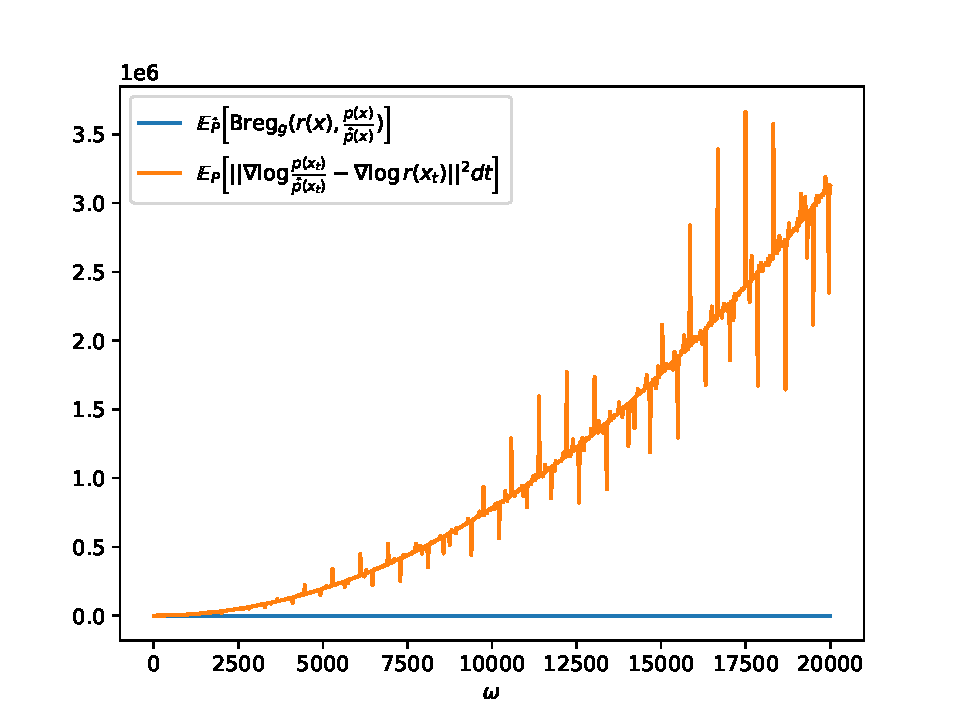
\includegraphics[width=0.8\linewidth]{gfx/1D_exple.pdf}
    \caption{1-dimensional example : Density ratio between two Gaussians, with a discriminator having an $\varepsilon$-optimal cross-entropy and a gain that goes to infinity}
    \label{fig:1Dexple}
\end{figure}







\subsection{Proof of Theorem~\ref{theorem:expectation_exploding}}\label{sec:app:proofoverfitting}


\begin{proof}
    Define the measures $\tilde{\mu}=\min\left(P,\hat{P}\right),\mu_{P}=\max\left(0,P-\hat{P}\right)$
    and $\mu_{\hat{P}}=\max\left(0,\hat{P}-P\right)$. Observe that $P=\tilde{\mu}+\mu_{P}$,
    $\hat{P}=\tilde{\mu}+\mu_{\hat{P}}$ and that $\tilde{\mu}\left(\mathbb{R}\right)=1-TV$
    where $TV$ is the total variation distance between $P$ and $\hat{P}$.
    Define the distribution $\mu=\frac{\tilde{\mu}}{\tilde{\mu}(\mathbb{R})}$
    and let $f_{\mu}$ and $f_{\tilde{\mu}}$ be the density of $\mu$
    and $\tilde{\mu}$ with respect to Lebesgue measure. Note that because
    $\tilde{\mu}$ is not normalized, $f_{\tilde{\mu}}$ does not integrate
    to one.
    
    Let us build two sets $S$ and $S'$ iteratively using the following
    rejection sampling procedure: First, start with $S=S'=\emptyset$.
    Then, for each $i$, add $x_{i}$ (respectively $x'_{i}$) to the
    set $S$ (respectively $S'$) with probability $\frac{f_{\tilde{\mu}}(x_{i})}{p(x_{i})}$
    (respectively $\frac{f_{\tilde{\mu}}(x'_{i})}{\hat{p}(x'_{i})}$).
    For now, denote $M_{1}=\left|S\right|$ and $M_{2}=\left|S'\right|$.
    It is easy to check using standard properties of rejection sampling
    that $\mathbb{E}\left[M_{1}\right]=\mathbb{E}\left[M_{2}\right]=N\times(1-TV)$.
    Finally, take the largest of both sets $S$ and $S'$ and remove its
    last added elements until both sets have same cardinality $M=\min\left(M_{1},M_{2}\right)$.
    Note that in all three sets $S$,$S'$ and $S\cup S'$, examples are
    distributed i.i.d. from $\mu$.
    
    Let us define the mean square error:
    
    \begin{align*}
    MSE & =\mathbb{E}_{x\sim P}\left[\left(\nabla_{x}d^{\star}(x)-\nabla_{x}d_{\phi}(x)\right)^{2}\right]\\
     & \ge\mathbb{E}\left[\left(\nabla_{x}d_{\phi}\right)^{2}\right]-2\mathbb{E}\left[\nabla_{x}d^{\star}.\nabla_{x}d_{\phi}\right]\\
     & \ge\mathbb{E}_{p}\left[\left(\nabla_{x}d_{\phi}\right)^{2}\right]-2\sqrt{\mathbb{E}_{p}\left[\left(\nabla_{x}d^{\star}\right)^{2}\right]}\sqrt{\mathbb{E}_{p}\left[\left(\nabla_{x}d_{\phi}\right)^{2}\right]}
    \end{align*}
    
    The last line follows from Cauchy-Schwartz inequality.
    
    We are interested into lower-bounding the \emph{expected} mean square
    error, noted $\mathbb{E}MSE$, where the expectation is over the training
    set $\left\{ x_{1},x_{1}'\ldots\right\} $ on which the discriminator
    $d_{\phi}$ is trained. So we would like to bound it.
    
    To derive this bound, we will first lower bound $\mathbb{E}_{p}\left[\left(\nabla_{x}d_{\phi}\right)^{2}\right]$.
    
    First, consider an arbitrary interval $B\subset\mathbb{R}$ of size
    $\beta$ containing at least one point $z\in S$ and one point $z'\in S'$
    such that $z<z'$.
    
    Then we can write
    
    \begin{align*}
    \int_{\mathbb{R}}\left(\nabla d_{\phi}\right)^{2}dP(x) & \ge\int_{B}\left(\nabla d_{\phi}\right)^{2}dP(x)\\
     & \ge\int_{B}\left(\nabla d_{\phi}\right)^{2}d\tilde{\mu}(x)=\int_{B}\left(\nabla d_{\phi}\right)^{2}f_{\tilde{\mu}}(x)dx\\
     & \ge\left(\inf_{x\in B}f_{\tilde{\mu}}(x)\right)\int_{B}\left(\nabla d_{\phi}\right)^{2}dx\\
     & \ge\left(\inf_{x\in B}f_{\tilde{\mu}}(x)\right)\int_{z}^{z'}\left(\nabla d_{\phi}\right)^{2}dx\\
     & =\left(\inf_{x\in B}f_{\tilde{\mu}}(x)\right)(z'-z)\int_{z}^{z'}\frac{\left(\nabla d_{\phi}\right)^{2}}{z'-z}dx\\
     & \ge\left(\inf_{x\in B}f_{\tilde{\mu}}(x)\right)(z'-z)\left(\int_{z}^{z'}\frac{\nabla d_{\phi}}{z'-z}dx\right)^{2}\text{ (by Jensen)}\\
     & =\frac{\inf_{x\in B}f_{\tilde{\mu}}(x)}{z'-z}\left(\int_{z}^{z'}\nabla d_{\phi}dx\right)^{2}\\
     & \ge\frac{\inf_{x\in B}f_{\tilde{\mu}}(x)}{\beta}\left(\int_{z}^{z'}\nabla d_{\phi}dx\right)^{2}
    \end{align*}
    
    Because both $p$ and $\hat{p}$ are L-Lipschitz, $f_{\tilde{\mu}}$
    has also this Lipschitz property. So for any $u\in B$ we have $f_{\tilde{\mu}}(u)-\inf_{x\in B}f_{\tilde{\mu}}(x)\le L\beta$,
    so $\inf_{x\in B}f_{\tilde{\mu}}(x)+L\beta\ge f_{\tilde{\mu}}(u)$,
    so $\inf_{x\in B}f_{\tilde{\mu}}(x)+L\beta\ge\frac{1}{\beta}\int_{B}f_{\tilde{\mu}}(x)dx=\frac{\tilde{\mu}\left(B\right)}{\beta}$.So
    we can write
    
    \[
    \int_{B}\nabla d_{\phi}^{2}dP(x)\ge\left(\frac{\tilde{\mu}\left(B\right)}{\beta^{2}}-L\right)\left(\int_{z}^{z'}\nabla d_{\phi}dx\right)^{2}
    \]
    
    Note that if $z>z'$ we would get by the same reasoning
    
    \[
    \int_{B}\nabla d_{\phi}^{2}dP(x)\ge\left(\frac{\tilde{\mu}\left(B\right)}{\beta^{2}}-L\right)\left(\int_{z'}^{z}\nabla d_{\phi}dx\right)^{2}
    \]
    
    To bound $\int_{z}^{z'}\nabla d_{\phi}dx$, recall that the cross-entropy
    for each $i$ is such that $\log\left(1+e^{-d_{\phi}(x_{i})}\right)\le\epsilon$
    and $\log\left(1+e^{d_{\phi}(x_{i}')}\right)\le\epsilon$. Thus,
    $1+e^{-d_{\phi}(x_{i})}\le e^{\epsilon}$ and $1+e^{d_{\phi}(x_{i}')}\le e^{\epsilon}$.
    So $d_{\phi}(x_{i})\ge\alpha$ and $d_{\phi}(x_{i}')\le-\alpha$
    where $\alpha=-\log\left(e^{\epsilon}-1\right)$. This also applies
    to $z$ and $z'$, so $\int_{\min(z,z')}^{\max(z,z')}\nabla d_{\phi}dx=\pm2\alpha$.
    Finally, we can summarize our findings by:
    
    \[
    \text{if both \ensuremath{S} and \ensuremath{S'} intersect with \ensuremath{B} then}\int_{B}\nabla d_{\phi}dP(x)\ge\left(\frac{\tilde{\mu}\left(B\right)}{\beta^{2}}-L\right)4\alpha^{2}
    \]
    
    Our goal now will be to show that there exists a small enough interval
    $B$ containing two points $z$ and $z'$ from $S$ and $S'$ with
    high probability.
    
    First, let us build an interval $A$ such that $\mu\left(A\right)\ge\frac{1}{2}$.
    By Chebyshev's inequality, we have that $\mu\left(\left\{ x:\left|x-\mathbb{E}_{\mu}x\right|\ge b\right\} \right)\le\frac{Var_{\mu}}{b^{2}}$
    for any $b$, so using the bound on the variance of lemma \ref{lem:variance_of_mu},
    we get that there exists a finite interval $A=\left[\mathbb{E}_{\mu}X-b,\mathbb{E}_{\mu}X+b\right]$
    where $b=\frac{\min\left(\sqrt{Var_{P}},\sqrt{Var_{\hat{P}}}\right)}{1-TV}$
    such that $\mu\left(A\right)\ge\frac{1}{2}$.
    
    Next, because $\mu(A)\ge\frac{1}{2}$, for any $0<\beta<2b$ there
    exists an interval $B\subset A$ of size $\beta$ such that $\mu\left(B\right)\ge\frac{\beta}{4b}$.
    Let us bound the probability that both $S$ and $S'$ intersect with
    $B$:
    
    \begin{align*}
    \mathbb{P}\left[B\cap S\neq\emptyset\wedge B\cap S'\neq\emptyset\right]= & 1-\mathbb{P}\left[B\cap S=\emptyset\vee B\cap S'=\emptyset\right]\\
    = & 1-\mathbb{P}\left[B\cap S=\emptyset\right]-\mathbb{P}\left[B\cap S'=\emptyset\right]+\mathbb{P}\left[B\cap S'=\emptyset\wedge B\cap S'=\emptyset\right]\\
    = & 1-\mu\left(\bar{B}\right)^{M}-\mu\left(\bar{B}\right)^{M}+\mu\left(\bar{B}\right)^{2M}\\
    \ge & 1-2\left(1-\mu\left(B\right)\right)^{M}\ge1-2\exp\left(-M\mu\left(B\right)\right)\\
    \ge & 1-2\exp\left(-\frac{M\beta}{4b}\right)
    \end{align*}
    
    For any non negative random variable $Z$, we know by the law of total
    expectation that $\mathbb{E}Z\ge\mathbb{E}\left[Z\mid condition\right]\mathbb{P}\left(condition\right)$,
    so in our case we have (here the expectation is over the dataset and
    the rejection sampling procedure):
    
    \begin{align*}
    \mathbb{E}\int_{B}\left(\nabla d_{\phi}\right)^{2}dP(x)\ge & \mathbb{E}\left[\int_{B}\left(\nabla d_{\phi}\right)^{2}dP(x)\mid B\cap S\neq\emptyset\wedge B\cap S'\neq\emptyset\right]\times\mathbb{P}\left[B\cap S\neq\emptyset\wedge B\cap S'\neq\emptyset\right]\\
    \ge & \left(\frac{\tilde{\mu}\left(B\right)}{\beta^{2}}-L\right)4\alpha^{2}\times\left(1-2\exp\left(-\frac{M\beta}{4b}\right)\right)\\
    \ge & \left(\frac{\mu\left(B\right)(1-TV)}{\beta^{2}}-L\right)4\alpha^{2}\times\left(1-2\exp\left(-\frac{M\beta}{4b}\right)\right)\\
    \ge & \left(\frac{1-TV}{4b\beta}-L\right)4\alpha^{2}\times\left(1-2\exp\left(-M\frac{\beta}{4b}\right)\right)
    \end{align*}
    
    Choosing $\beta=\frac{b}{M}4\log4$ we get a $\left(1-2\exp\left(-M\frac{\beta}{4b}\right)\right)=1/2$
    and 
    \begin{align*}
    \mathbb{E}\int_{B}\left(\nabla d_{\phi}\right)^{2}dP(x) & \ge\mathbb{E}\left(\frac{1-TV}{4b\beta}-L\right)2\alpha^{2}\\
     & =\left(\frac{(1-TV)\mathbb{E}\left[M\right]}{8b^{2}\log4}-2L\right)\left(\log\left(e^{\epsilon}-1\right)\right)^{2}
    \end{align*}
    
    It is known that $\mathbb{E}M=\mathbb{E}\min\left(M_{1},M_{2}\right)\ge\frac{1}{2}\mathbb{E}M_{1}=\frac{N\times(1-TV)}{2}$.
    So we finally get\\
    \begin{align*}
    \mathbb{E}\int_{\infty}\left(\nabla d_{\phi}\right)^{2}dP(x) & \ge\left(N\frac{(1-TV)^{2}}{16b^{2}\log4}-2L\right)\left(\log\left(e^{\epsilon}-1\right)\right)^{2}\\
     & =\left(N\frac{(1-TV)^{4}}{16\log4\min\left(Var_{P},Var_{\hat{P}}\right)}-2L\right)\left(\log\left(e^{\epsilon}-1\right)\right)^{2}
    \end{align*}
    
    Finally, we can bound the expected MSE:
    
    \begin{align*}
    \mathbb{E}MSE & \ge\mathbb{E}_{p}\left[\left(\nabla_{x}d_{\phi}\right)^{2}\right]-2\sqrt{\mathbb{E}_{p}\left[\left(\nabla_{x}d^{\star}\right)^{2}\right]}\sqrt{\mathbb{E}_{p}\left[\left(\nabla_{x}d_{\phi}\right)^{2}\right]}\\
     & \ge\mathbb{E}_{p}\left[\left(\nabla_{x}d_{\phi}\right)^{2}\right]-2\sqrt{\mathbb{E}_{p}\left[\left(\nabla_{x}d^{\star}\right)^{2}\right]}\sqrt{\mathbb{E}_{p}\left[\left(\nabla_{x}d_{\phi}\right)^{2}\right]}\\
    \end{align*}
    \end{proof}
    \begin{lemma}
    \label{lem:variance_of_mu}Let $P$ and $\hat{P}$ be two distributions
    over $\mathbb{R}$ and let $\tilde{\mu}=\min\left(P,\hat{P}\right)$.
    Then 
    \[
    Var_{\mu}\le\frac{1}{2(1-TV)^{2}}\min\left(Var_{P},Var_{\hat{P}}\right)
    \]
    \end{lemma}
    
    
    \begin{proof}
    Define $\mu=\frac{\tilde{\mu}}{\tilde{\mu}(\mathbb{R})}$. As before,
    $\mu=\frac{\tilde{\mu}}{1-TV}$, so we have
    
    \begin{align*}
    Var_{\mu} & =\mathbb{E}_{X\sim\mu}\left[(X-\mathbb{E}X)^{2}\right]=\frac{1}{2}\mathbb{E}_{X,X'\sim\mu}\left[(X-X')^{2}\right]\\
     & =\frac{1}{2}\int\int(x-x')^{2}d\mu(x)d\mu(x')\\
     & =\frac{1}{2(1-TV)^{2}}\int\int(x-x')^{2}d\tilde{\mu}(x)d\tilde{\mu}(x')\\
     & \le\frac{1}{2(1-TV)^{2}}\min\left(\int\int(x-x')^{2}dpdp,\int\int(x-x')^{2}d\hat{p}d\hat{p}\right)\\
     & =\frac{1}{2(1-TV)^{2}}\min\left(Var_{P},Var_{\hat{P}}\right)
    \end{align*}
    \end{proof}
    

    \subsection{Proof of Proposition~\ref{theorem:optimality_mse_sm}}\label{sec:app:proofmseloss}

\begin{proposition}
    Assume that $P$ and $\whP$ satisfy the assumptions detailed in Appendix~\ref{sec:appendix:assumptionssong}.
    Then, the following holds:
    \begin{equation}
        \argmin_\phi \calL_{\mathrm{SM}}^{d}(\phi) = \argmin_\phi \calL_{\mathrm{MSE}}^{d}(\phi).
    \end{equation} 
\end{proposition}
First, we can show that:
\begin{align}
    \calL_{\mathrm{MSE}}^{d}(\phi) =& \int_0^T\lambda(t)   \E_{P_0, P_{t\vert\vx_0}}\left[\Vert \nabla_{\vx_t} \log p_t(\vx_t\vert\vx_0) - \nabla_{\vx_t} \log \whp_t(\vx_t) - \nabla_{\vx_t} \vd_\phi(\vx_t, t)\Vert_2^2 \right]\dt \\
    =& \begin{aligned}[t]
        \int_0^T&\lambda(t) \E_{P_t}\left[\frac{1}{2}\left\Vert\nabla_{\vx_t} \vd_\phi(\vx_t, t)\right\Vert_2^2\right] \dt \\
        &+ \int_0^T\lambda(t) \E_{P_0, P_{t\vert\vx_0}}\left[\left\langle \nabla_{\vx_t}d(\vx_t, t), \nabla_{\vx_t} \log \frac{p_t(\vx_t\vert\vx_0)}{\whp_t(\vx_t)}\right\rangle\right] \dt \\
        &+ \int_0^T\lambda(t) \E_{P_0, P_{t\vert\vx_0}}\left[\frac{1}{2}\left\Vert\nabla_{\vx_t} \log \frac{p_t(\vx_t\vert\vx_0)}{\whp_t(\vx)}\right\Vert_2^2\right] \dt 
    \end{aligned}\\
    =& \int_0^T\lambda(t) \E_{P_t}\left[\frac{1}{2}\left\Vert\nabla_{\vx_t} \vd_\phi(\vx_t, t)\right\Vert_2^2\right] \dt + J(\phi) + C_1,
\end{align}
where $C_1$ is a constant independent of $\phi$. And we can write $J$ as:
\begin{align}
    J(\phi) =& \int_0^T\lambda(t) \E_{P_0, P_{t\vert\vx_0}}\left[\left\langle \nabla_{\vx_t}d(\vx_t, t), \nabla_{\vx_t} \log \frac{p_t(\vx_t\vert\vx_0)}{\whp_t(\vx_t)}\right\rangle\right] \dt \\
    =& \begin{aligned}[t]
       \int_0^T&\lambda(t) E_{P_0, P_{t\vert\vx_0}}\left[\left\langle \nabla_{\vx_t}d(\vx_t, t), \nabla_{\vx_t} \log p_t(\vx_t\vert\vx_0)\right\rangle\right] \dt \\
        &- \int_0^T\lambda(t) E_{P_0, P_{t\vert\vx_0}}\left[\left\langle \nabla_{\vx_t}d(\vx_t, t), \nabla_{\vx_t} \log \whp_t(\vx_t)\right\rangle\right] \dt. 
    \end{aligned} 
\end{align}
Using the result of \citep{vincent_connection_2011}, we can show the term in the first integral can be rewritten as:
\begin{align}
    E_{P_0, P_{t\vert\vx_0}}\left[\left\langle \nabla_{\vx_t}d(\vx_t, t), \nabla_{\vx_t} \log p_t(\vx_t\vert\vx_0)\right\rangle\right] =  E_{P_t}\left[\left\langle \nabla_{\vx_t}d_\phi(\vx_t, t), \nabla_{\vx_t} \log p_t(\vx_t)\right\rangle\right].
\end{align}
Thus, we can rewrite $J$ as:
\begin{align}
    J(\phi) =& \begin{aligned}[t]
        \int_0^T&\lambda(t) E_{P_t}\left[\left\langle \nabla_{\vx_t}d_\phi(\vx_t, t), \nabla_{\vx_t} \log p_t(\vx_t)\right\rangle\right] \dt \\
        &- \int_0^T\lambda(t) E_{P_0, P_{t\vert\vx_0}}\left[\left\langle \nabla_{\vx_t}d(\vx_t, t), \nabla_{\vx_t} \log \whp_t(\vx_t)\right\rangle\right] \dt
    \end{aligned} \\
    = & \int_0^T\lambda(t) E_{P_t}\left[\left\langle \nabla_{\vx_t}d_\phi(\vx_t, t),\nabla_{\vx_t} \log \frac{p_t(\vx_t)}{\whp(\vx_t)}\right\rangle\right] \dt.\label{eq:J}
\end{align}
And on the other side, we have:
\begin{align}
    \calL_{SM}^d(\phi) =& \int_0^T\lambda(t) \E_{P_t}\left[\Vert \nabla_{\vx_t} \vd_\phi(\vx_t, t)\Vert_2^2\right] \dt \\
    =& \begin{aligned}[t]
        \int_0^T&\lambda(t) \E_{P_t}\left[\frac{1}{2}\left\Vert\nabla_{\vx_t} \vd_\phi(\vx_t, t)\right\Vert_2^2\right] \dt \\
        &+ \int_0^T\lambda(t) \E_{P_t}\left[\left\langle \nabla_{\vx_t}d(\vx_t, t), \nabla_{\vx_t} \log \frac{p_t(\vx_t)}{\whp_t(\vx_t)}\right\rangle\right] \dt \\
        &+ \int_0^T\lambda(t) \E_{P_t}\left[\frac{1}{2}\left\Vert\nabla_{\vx_t} \log \frac{p_t(\vx_t)}{\whp_t(\vx_t)}\right\Vert_2^2\right] \dt
    \end{aligned} \\
    =& \int_0^T\lambda(t) \E_{P_t}\left[\frac{1}{2}\left\Vert\nabla_{\vx_t} \vd_\phi(\vx_t, t)\right\Vert_2^2\right] \dt + J(\phi) + C_2 
\end{align}
using Equation~\eqref{eq:J} and $C_2$ is a constant independent of $\phi$. Thus, we have $\calL_{\mathrm{MSE}}^{d}(\phi) = \calL_{\mathrm{SM}}^{d}(\phi) + C_3$, where $C_3$ is a constant independent of $\phi$. Thus, the minimizer of $\calL_{\mathrm{MSE}}^{d}(\phi)$ is the same as the minimizer of $\calL_{\mathrm{SM}}^{d}(\phi)$.
\cleardoublepage

% **************************************************
% End of Document CONTENT
% **************************************************
\end{document}
